\documentclass[10pt]{beamer}
\usetheme[
%%% options passed to the outer theme
%    progressstyle=movCircCnt,   %either fixedCircCnt, movCircCnt, or corner
%    rotationcw,          % change the rotation direction from counter-clockwise to clockwise
%    shownavsym          % show the navigation symbols
  ]{AAUsimple}
  
% If you want to change the colors of the various elements in the theme, edit and uncomment the following lines
% Change the bar and sidebar colors:
%\setbeamercolor{AAUsimple}{fg=red!20,bg=red}
%\setbeamercolor{sidebar}{bg=red!20}
% Change the color of the structural elements:
%\setbeamercolor{structure}{fg=red}
% Change the frame title text color:
%\setbeamercolor{frametitle}{fg=blue}
% Change the normal text color background:
%\setbeamercolor{normal text}{fg=black,bg=gray!10}
% ... and you can of course change a lot more - see the beamer user manual.

\usepackage[utf8]{inputenc}
\usepackage[english]{babel}
\usepackage[T1]{fontenc}
% Or whatever. Note that the encoding and the font should match. If T1
% does not look nice, try deleting the line with the fontenc.
\usepackage{helvet}
\usepackage{graphicx} %For figures
\graphicspath{{./images/}}
\usepackage{tikz} %Tikz
\usepackage{tikzscale}
\usepackage{tikz-uml}
\usepackage{framed}
\usetikzlibrary{calc, arrows, decorations.markings,decorations.text, shapes, positioning, decorations.pathreplacing}
\usepackage{pgfplots} %Graph plotting
\pgfplotsset{compat=newest,
  table/col sep = comma,
  every axis legend/.append style={
    no marks,
    filter discard warning=false,
  }
}
\usepackage{siunitx}

\usepackage{subfig}
\usepackage{tcolorbox}
\usepackage{xcolor}

\usepackage{import}

% colored hyperlinks
\newcommand{\chref}[2]{%
  \href{#1}{{\usebeamercolor[bg]{AAUsimple}#2}}%
}
\newcommand{\perc}[1]{\SI{#1}{\percent}}
\renewcommand{\arraystretch}{1.25}

\title{Point and Control with Gestures in a Smart Home}

% \subtitle{v.\ 1.3.2}  % could also be a conference name

\date{\today}

\author{
  Jens Emil Gydesen\\ \href{mailto:jgydes11@student.aau.dk}{{\tt jgydes11@student.aau.dk}}\\
  Kasper Lind Sørensen\\  \href{mailto:klsa11@student.aau.dk}{{\tt klsa11@student.aau.dk}}\\
  Simon B. Støvring\\ \href{mailto:sstavr11@student.aau.dk}{{\tt sstavr11@student.aau.dk}}
}

%Brug til header:
\newcommand{\authornames}{Jens Emil Gydesen, Kasper Lind Sørensen and Simon B. Støvring}

% - Give the names in the same order as they appear in the paper.
% - Use the \inst{?} command only if the authors have different
%   affiliation. See the beamer manual for an example

\institute[
%  {\includegraphics[scale=0.2]{aau_segl}}\\ %insert a company, department or university logo
  Dept.\ of Computer Science\\
  Aalborg University\\
  Denmark
] % optional - is placed in the bottom of the sidebar on every slide
{% is placed on the bottom of the title page
  Department of Computer Science\\
  Aalborg University\\
  Denmark
  
  %there must be an empty line above this line - otherwise some unwanted space is added between the university and the country (I do not know why;( )
}

% specify a logo on the titlepage (you can specify additional logos an include them in 
% institute command below
\pgfdeclareimage[height=1.5cm]{titlepagelogo}{AAUgraphics/aau_logo_new} % placed on the title page
%\pgfdeclareimage[height=1.5cm]{titlepagelogo2}{AAUgraphics/aau_logo_new} % placed on the title page
\titlegraphic{% is placed on the bottom of the title page
  \pgfuseimage{titlepagelogo}
%  \hspace{1cm}\pgfuseimage{titlepagelogo2}
}

\begin{document}
% the titlepage
{\aauwavesbg%
\begin{frame}[plain,noframenumbering] % the plain option removes the header from the title page
  \titlepage
\end{frame}}
%%%%%%%%%%%%%%%%

% TOC
\begin{frame}{Agenda}{}
\tableofcontents
\end{frame}
%%%%%%%%%%%%%%%%

\chapter{Introduction}\label{chap:introduction}
\todo{Write introducing text to introduction chapter}
\section{Wearables}\label{sec:wearables} %Working title
%Thalley: Første source kan også laves som en fin graf hvis ønsket. Brug tal fra: http://www.statista.com/statistics/259372/wearable-device-market-value/
Wearable technology is a trending form of technology as of 2015 \cite{WEARABLESTREND}. 
As the name implies, wearables are devices that, unlike most electronics, are worn by the user. 
The most common types of wearables today are smartwatches, 
\ie watches that run an advanced operating system and can perform more actions that regular watches such as communicating with a smartphone or other smart devices, 
and smart wristbands which usually tracks activity, 
among other things, and sends this data to a connected smartphone via an application. 
Smartphones are usually not considered a wearable since they are usually \emph{carried} and not \emph{worn}. 

%Hvorfor wearables?
The increasing trend in wearables is likely due to increased computational power in small devices and decreased sizes of sensors, 
which allows more power and functionality to wearables devices. 
The increasing trend, as well as better wearables devices, 
opens up new possibilities since we can now carry more computational power with us on the go that we can utilize to perform actions that we could not before, 
or perform other actions faster or better. 
Examples of this could be that we can now track our level of activity together with our location to analyze ourselves or even automate actions based on our location, mood or even health. 

%HVad kan en wearable? Hvilke sensorer findes der? Hvad er state of the art? 
If we take a look at some of the current state of the art or the most popular wearable devices right now, 
we can create an image of what we can actually monitor, track, control or in other ways do with devices that we can wear. 
One of the latest and most advanced wearable is the HIRIS \cite{hirisweb}. 
The HIRIS is a wearable computer able to track 3D movements in real-time. 
By using several HIRIS, you can get a create a full-body tracking system. 
Aside from 3D tracking, HIRIS also tracks heart rate and temperature and can connect to other devices and control these. 
Another advanced wearable tracker is the Jawbone UP3 \cite{JAWBONE}. 
This wearable is also able to track your heart rate, activity, sleep and temperature, but unlike the Hiris cannot control any other devices. 
Since one of the most popular wearables is the smartwatch, it makes sense to mention these as well. 
One of most interesting smartwatches, due to developer options, is the Pebble Smartwatch \cite{PEBBLE}. 
This smartwatch works with iPhones and Android smartphones and comes with a variety of applications for tracking fitness and control music among other things. 
Aside from this, the watch also comes with an accelerometer and a magnetometer, meaning that is can track your motions and directions. 

By analyzing the list of 348 different wearables from Vandrico\cite{LISTOFWEARABLES} of September 2015, 
we can see which sensors and components are most common among wearables and where on the body they are worn. 
It is important to note that all of this information comes Vandrico's database, and may differ from other findings. 
\Cref{fig:wearables-category} shows which categories these wearables fit in. The most common one, lifestyle, 
describes wearables such as smartwatches or other devices that are meant to be used and worn on a daily basis. 
Some devices may fit more than one category.

\begin{figure}[!htb]
    \centering
    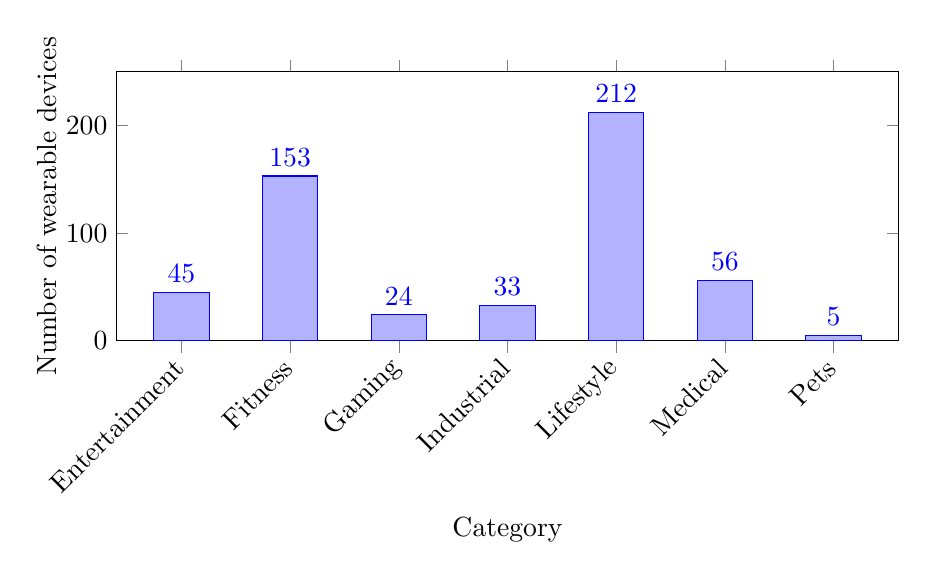
\begin{tikzpicture}
    \begin{axis}[
        height=5cm,
        width=0.95\textwidth,
        xlabel={Category},
        xticklabel style={rotate=45, anchor=east, yshift=-0.5ex},
        ylabel={Number of wearable devices},
        yticklabel style={align=right,inner sep=0pt,xshift=-0.3em},
        nodes near coords align={vertical},
        nodes near coords,
        xtick=data,
        symbolic x coords={Entertainment,Fitness,Gaming,Industrial,Lifestyle,Medical,Pets},
        ybar,
        ymax=250,
        ymin=0,
        bar width=20pt,
        ]
        \addplot coordinates {(Entertainment,45) (Fitness,153) (Gaming,24) (Industrial,33) (Lifestyle,212) (Medical,56) (Pets,5)};
    \end{axis}
\end{tikzpicture}
    \caption{Number of devices in each category}
    \label{fig:wearables-category}
\end{figure}

\Cref{fig:wearables-placement} shows where on the body the wearable should or can be worn. 
The most common placement is the wrist where smartwatches or wristband are worn, 
which are the most popular wearables. The devices that are worn on the head are usually augmented/virtual reality headsets, 
but also includes smart bike-helmets or ear/headphones.

\begin{figure}[!htb]
    \centering
    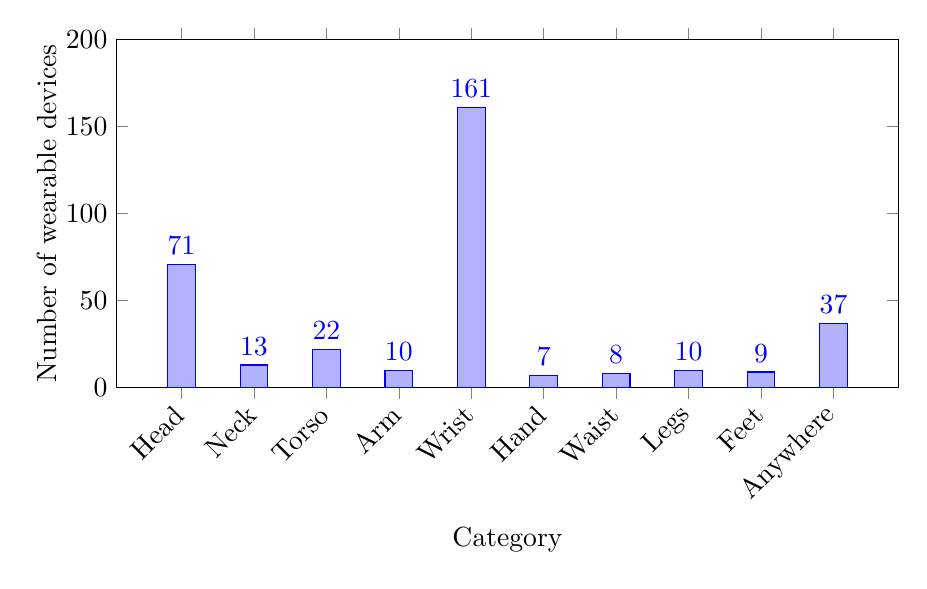
\begin{tikzpicture}
\begin{axis}[
    height=6cm,
    width=0.95\textwidth,
    xlabel={Category},
    xticklabel style={rotate=45, anchor=east, yshift=-0.5ex},
    ylabel={Number of wearable devices},
    yticklabel style={align=right,inner sep=0pt,xshift=-0.3em},
    nodes near coords align={vertical},
    nodes near coords,
    xtick=data,
    symbolic x coords={Head,Neck,Torso,Arm,Wrist,Hand,Waist,Legs,Feet,Anywhere},
    ybar,
    ymax=200,
    ymin=0,
    ]
    \addplot coordinates {(Head,71) (Neck,13) (Torso,22) (Arm,10) (Wrist,161) (Hand,7) (Waist,8) (Legs,10) (Feet,9) (Anywhere,37)};
\end{axis}
  

\end{tikzpicture}
    \caption{Placements of wearables}
    \label{fig:wearables-placement}
\end{figure}

\Cref{fig:wearables-sensors} shows which sensors and components are mostly available in wearables. 
Due to its high usability, the accelerometer is a very important sensor which is found in approximately half the wearables. 
The remaining sensors in \Cref{fig:wearables-sensors} are, unsurprisingly sensors that we also find in smartphones as they give a lot of options when it comes to developing applications. 
\begin{figure}[!htb]
    \centering
    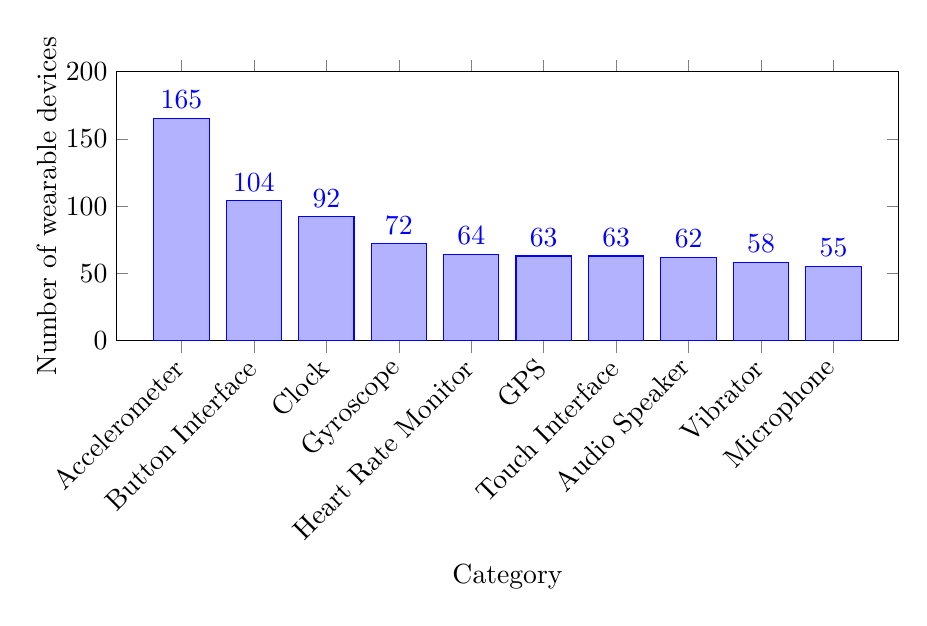
\begin{tikzpicture}
    \begin{axis}[
        height=5cm,
        width=0.95\textwidth,
        xlabel={Category},
        xticklabel style={rotate=45, anchor=east, yshift=-0.5ex},
        ylabel={Number of wearable devices},
        yticklabel style={align=right,inner sep=0pt,xshift=-0.3em},
        nodes near coords align={vertical},
        nodes near coords,
        xtick=data,
        symbolic x coords={Accelerometer,Button Interface,Clock,Gyroscope,Heart Rate Monitor,GPS,Touch Interface,Audio Speaker,Vibrator,Microphone},
        ybar,
        ymax=200,
        ymin=0,
        bar width=20pt,
        ]
        \addplot coordinates {(Accelerometer,165) (Button Interface,104) (Clock,92) (Gyroscope,72) (Heart Rate Monitor,64) (GPS,63) (Touch Interface,63) (Audio Speaker,62) (Vibrator,58) (Microphone,55)};
    \end{axis}
\end{tikzpicture}
    \caption{Top 10 mostly used sensors}
    \label{fig:wearables-sensors}
\end{figure}

This section gave a short overview of the current state of wearables, what they are and which sensors are widely available. 
This information should be remembered if developing any system that utilizes wearables. 

%Skab et overblik over de nyeste devices
%Grafer over hvilke sensorere der mest typiske?
%Grafer over kropsdele?
%Hvad er de nyeste teknologier indenfor wearables? 

\section{Smart Homes}
Another trend that utilizes the concept of IoT is smart homes which are homes that are, 
to some degree, automated by utilization IoT devices. 
The devices used for smart homes differ greatly from wearables as they are usually stationary. 
The concept of smart homes have been around for a while and numerous homes have already integrated some of these smart devices. 
A good example of a high-end smart home is Bill Gate's mansion in Medina, Washington \cite{billgatehouse}.
This \$100 million house have sensors to adjust each room's temperature and lighting, 
and have speakers behind the wallpaper that follows you from room to room. 
The artwork in the house is mostly digital and can be changed by pressing a button. 
One can only imagine what other technology is being used in that house. 

However, that is a rather extreme example of a smart home. 
Ordinarily, the devices found in smart homes are common items that has been connected to the Internet for wireless control.
Common devices that are found in smart homes include, but are not limited to, 
coffee machines, washers and dryers, thermostats, sound systems and locks. 
However, only few devices have really gained ground for the common user and few homes are automated.
One of the most commonly found IoT in homes are the Nest thermostat \cite{NEST}. 
This thermostat senses when you are around and when you are not to control the climate inside to save energy and thus money.
Unlike a lot of smart devices that are made to make your life a little easier, such as an automated coffee machine, 
the Nest thermostat helps you save money which is likely the reason for it popularity. 
Furthermore, the newest version (as of October 2015) allows you to connect other IoT devices to the thermostat. 
The Nest thermostat is thus starting to solve what is probable the greatest problem with smart homes (and IoT in general), 
and why they have not become popular yet: Lack of interconnectivity between IoT devices. 
This problem leads us to what is known as smart hubs. 

\subsection{Smart Hubs}
A smart hub is a device, or service, that implements several communication protocols used by IoT devices, 
and gives the user a single protocol or interface. 
The goal of a smart hub is to make the connected devices able to communicate. 

\subsubsection{Common Protocols for IoT}
\todo[author=Thalley]{Insert figure illustrating this}
There is a range of different protocols that are being used for various smart devices. 
We will not get into much detail with these protocols, 
but we demonstrate how many different there are and why communication is a problem.
\begin{table}
   \begin{description}
       \item[Protocol:] ZigBee
       \item[Used by:] Samsung, Jasco, Smartenit, FortrezZ and others
       \item[In products:] SmartThings Hub, thermostats, door sensors, light bulbs, etc.\\
       
       \item[Protocol:] Z-Wave
       \item[Used by:] FortrezZ, GE, Intermatic, Leviton, Aeon Labs, Evolve and others
       \item[In products:] Thermostats, wall outlets, door locks, door and window sensors, etc.  \\
       
       \item[Protocol:] WiFi (IEEE 802.11)
       \item[Used by:] Nest, Philips, Samsung, Bose, D-link and others
       \item[In products:] Thermostats, speakers, light bulbs, motion sensors, fitness trackers, camera, etc. 
    \end{description}
    \caption{Protocols used by various IoT devices}\label{table:iotprotocols}
\end{table}

Aside from the protocols in \Cref{table:iotprotocols}, 
there are several others messaging protocols such as MQTT, CoAP and XMPP used by various devices. 

A smart hub should thus not only be able to communicate with the devices, 
but also be able to transform the data to a single format and give easy access to it. 

\subsubsection{Smart Hubs on the Market}
The requirements for smart hubs have gained the attention of several large companies and even more smaller companies, 
all competing to be center of future smart homes. 
One of the mature commercial available smart hubs is the Samsung SmartThings Hub\cite{SMARTTHINGS}. 
The SmartThings Hub is a standalone device that supports the Z-Wave, ZigBee and WiFi protocols, 
and provides a smartphone application or a Representational State Transfer (REST) interface. 
The SmartThings Hub has been tested and is compatible with more than 150 devices as of October 2015,
but with support for the aforementioned protocols and a REST interface, this number is in practice higher.  
The price for such a hub is \$99, which is, compared to the prices for some of the compatible devices, very affordable. 
A more detailed description of the Samsung SmartThings Hub can be found in \Cref{sec:smartthings}. 

Samsung is, however, not the only company selling smart hubs. 
Microsoft has been working on their HomeOS\cite{HOMEOS}, Apple has their HomeKit\cite{HOMEKIT} and Google recently announced Brillo\cite{BRILLO}. 
While these products differ in terms of architecture, descriptions (operating system contra hub) and availability,
they all share the same goal of giving a centralized control of smart devices. 

There are also other open source alternatives such as openHAB\cite{OPENHAB}, 
where you simply setup your own server running the open sourced code and control the devices through that. 
The advantage here is of course the price (free) and the possibility of adding new unsupported products. 

\Cref{table:smarthubs} gives a short overview of some of the available or coming smart hubs. 
\begin{table}
    \centering
    \begin{tabular}{l l}
        Company                           & Product                              \\\hline
        openHAB\cite{OPENHAB}             & Employ open source code on own server \\
        Open Source Automation\cite{OSA}  & Employ open source code on own server \\
        OpenRemote\cite{OPENREMOTE}       & Employ open source code on own server \\
        Apple\cite{HOMEKIT}               & HomeKit Framework \\
        Samsung\cite{SMARTTHINGS}         & SmartThings Hub: A standalone device that cost \$99 \\
        Microsoft\cite{HOMEOS}            & HomeOS: An Operating system that runs on a server \\
        Google\cite{BRILLO}               & Project Brillo: An Operating system that runs on a server
    \end{tabular}
    \caption{An overview of home automation hubs from different companies}
    \label{table:smarthubs}
\end{table}

\subsection{Control of Smart Homes}
While smart hubs let different smart devices communicate, 
they are not meant to be a control panel for smart homes (although some, such as HomeOS, is designed as such).
To control the devices connected to a smart home, or standalone smart devices, 
most vendors offer some sort of smartphone application that gives the consumer a basic interface to control the device, set rules for it and so on.
This is for example the case with the Samsung SmartThings hubs. 

An alternative to such an application could be the Logitech Harmony Remote\cite{HARMONYREMOTE}, 
which is a universal remote that can connect to over \num{270000} devices (smart and dumb). 
It comes either as a standalone remote control or connected with a hub. 

Gesture control is a newer and more advanced way of controlling a smart home. 
A company known as Reemo\cite{Reemo}, formerly Playtabase, has created a way of controlling smart devices by gestures. 
They have developed a wearable devices, located on the wrist, that allows user to point at a device, 
and then perform a pre-programmed gesture that corresponds to a certain action for that device. 
A small received has to be placed near the devices that you want to control, 
and it is this received that you have to point to as depicted by \Cref{fig:reemo}. 
The pointing will, however, only work if the device is within line of sight. 

\begin{figure}[!htb]
    \centering
    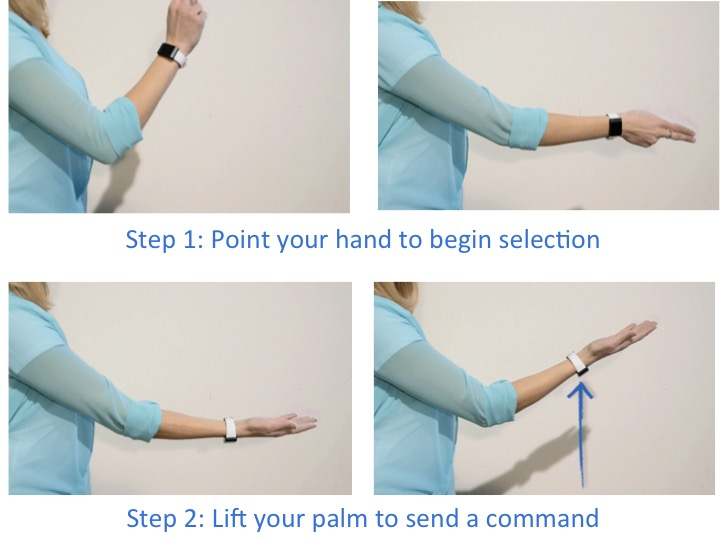
\includegraphics[width=0.8\textwidth]{images/Reemo}
    \caption{How Reemo gesture control works. Source: \url{http://www.getreemo.com/projects/}}
    \label{fig:reemo}
\end{figure}

Unfortunately they have not disclosed any details regarding the technology, 
how the receivers know which receiver you are pointing at or how the devices are controlled. 
The company and the product is also still in a development phase, 
so the product is not commercialized yet but have been in development since mid-2014.

These are the most common and/or most intuitive ways of controlling smart devices. 
The question is which is ``the best'', or rather, which method is the wanted way of controlling the devices.
\Cref{tbl:smartcontrol} summaries the aforementioned 3 ways. 

\begin{table}[!htb]
    \centering
    \parbox[t][][t]{0.3\textwidth}{
        \textbf{Smartphone application}\\
        \textbf{Pros:} Easy control of smart devices if the smartphone is usually carried or always near. 
                       Applications are usually available from vendors. 
                       Easy to get updates to the software. \\
        \textbf{Cons:} Requires a smartphone nearby to control. 
                       An overhead of unlocking phone, opening application and selecting device and action.
    }\quad
    \parbox[t][][t]{0.3\textwidth}{
        \textbf{Remote Control}\\
        \textbf{Pros:} Easy control of smart devices if the remote is usually carried or always near. \\
        \textbf{Cons:} Requires a remote control nearby to control (usually not very expensive). 
                       An overhead of selecting device and action.
    }\quad
    \parbox[t][][t]{0.3\textwidth}{
        \textbf{Gesture Control}\\
        \textbf{Pros:} Wearables are usually worn and grants easy control of applications by gesture.
                       Intuitive way of controlling devices (gestures imitates regular actions).
                       Easy to get updates to the software. 
                       No overhead of opening an application\\
        \textbf{Cons:} Requires a wearable to control. 
                       Have to remember gestures.
                       Must be in line of sight. 
    }
    \caption{Ways of controlling smart devices}
    \label{tbl:smartcontrol}
\end{table}

Each way has its pros and cons. 
A survey of 37 people showed that \perc{76} found gestures to be a natural way of controlling devices, 
while \perc{8} found it unnatural and the remaining left the question unanswered\cite{Kela2006}. 
This survey shows that users would rather have gesture for control, 
rather than the bother of always using their smartphone or remote for control.  
A product such as Reemo is a good way of controlling smart devices. 
However, as mentioned, it has a downside that the objects have to be in line of sight. 
If this restriction could be removed, it would improve this method. 

%%% Local Variables:
%%% mode: latex
%%% TeX-master: "../../master"
%%% End:

\section{Levels of Smart Home Automation}\label{sec:system-categories}
\todo[author=Thalley]{Bør vi ændre det med categories til noget med levels i stedet?}
Smart home automation is one of the big sell-points of smart homes.
Home automation can happen at various degrees. 
In this section we will analyze and categorize the different types of smart home automation. 
We divide the scenarios in which home automation is facilitated, 
into the following three categories:

\begin{enumerate}
    \item Rule driven systems
    \item Gesture driven systems
    \item Autonomous systems
\end{enumerate}

``Manual systems'' could constitute a fourth category, consisting of regular systems with manual switches,
but is left out as it such systems do not contribute to home automation.
The categories varies in the way users configure and interact with the systems. 
All the systems are, however, all driven by a set of \emph{rules}. 
The main difference is how the rules are defined or how they are used.
Each of the three categories and their use cases are briefly described below,
as well as how they can be integrated with wearables.

\subsection{User Defined Rule Systems}

These types of systems have a set of \emph{used defined} rules, 
that controls what the system does when certain events happen. 
The user defined rule systems use conditional statements to express input and output. 
Below are a few examples of rules in the form of (if this) \textrightarrow~(then that):

\begin{itemize}
    \item (The temperature is above 23 degrees Celsius) \textrightarrow~(Turn on the air conditioner)
    \item (The CO\textsubscript{2} index is critically high) \textrightarrow~(Open my windows)
\end{itemize}

The above rules consist of a condition on the left-hand side of the arrow, 
and an action on the right-hand side of the arrow.
The automation of the smart home is based on the set of rules. 
To achieve the desired behavior, the user must add, remove or tweak existing rules.

Examples of user defined rule systems include the aforementioned Apple HomeKit. 
As outlined in the framework reference for HomeKit \cite{applehomekitref}, 
the system is based on actions and events. 
Triggers constitutes rules by encapsulating actions and events. 
Each event represents a condition. 
An event may be fulfilled by a change in time, 
the state of devices in the system of the location of the user.

A wearable here could be integrated as a form of sensor (to \eg measure body temperature or CO\textsubscript{2} index), 
and use this information to perform the actions based on the rules.
Wearables could also be used to create a ``Follow Me'' system, 
that could track if the user is near \eg a door, and automatically open the door for the user. 

\subsection{Interactive Systems}

Interactive systems are explicitly controlled by the users, but in a smart way. 
Two main examples of interactive systems are gesture controlled and remote controlled. 

The gesture controlled systems are controlled by tracking the user's movements, 
and perform certain actions based on the movements.
Each device in the system responds to a set of gestures. 
For example, a lamp may respond to the user waving in order to turn on, 
and the user clapping in order to turn off.

A gesture driven system is partly a user defined rule system, 
as each gesture registered in the system is associated with one or more actions.
The association means that each time the gesture is registered in the system, the action should be triggered. 
Such rules can be formulated as ``if I wave, then lower the temperature on my thermostat'
The difference between these types of systems and the user defined rule systems, 
is that the actions are performed explicitly by the user, 
and not by measurements or other observations.

Examples of gesture driven systems include the aforementioned Hiris and Reemo, 
where wearables are used as active control units by performing gestures. 

The other type of interactive systems are the remove controlled systems. 
In these types of systems, the user controls the devices in the smart home using a remote control. 
The remote control could be the aforementioned Logitech Harmony Remote, 
but could also simply be a smartphone application. 
These types of systems are usually not combined with wearables, 
as they typically require a screen to control which device to perform an action on. 

\subsection{Autonomous Systems}

An autonomous system monitors the system, 
and proactively responds to changes in the system. 
Observable changes include but are not limited to changes in the temperature, 
CO\textsubscript{2} index, the number of people in the room or even who are in the room.
Autonomous systems should intelligently react to the users needs, 
based upon the observable state of the environment.

Autonomous systems rely on the concept of ambient intelligence, 
in order to determine the necessary actions.
\todo[author=Thalley]{Maybe add something about ambient intelligence here?}
Such systems include autonomous enhancement services, 
that replaces manual care with an automated system \cite{nehmer2006living}. 
These systems gather environment and user data, 
to determine the user's future actions or intentions. 
The autonomous systems are designed to what the users' want, 
without the users input or interaction. 
These systems applies methods and theories of statistics and machine learning, 
in order to learn the users behaviors and how to determine what the users want. 
For example if a user usually makes coffee in the morning, 
the system learns this routine and can then start the brewing process, 
when it measures that the user is waking up in the morning. 
%Thalley: Bedre eksempel ville være nice

Autonomous systems depend on rules like the previous two systems mentioned. 
The main difference here is that autonomous system create these rules \emph{themselves}, 
from observing the users and the environment, 
or with some preprogrammed rules defined by \emph{experts}
The rules of such systems are typically much more complex however. 
It is not given that users themselves are capable of determining a suitable set of rules, 
in order to \eg judge if their health is critical. 

\todo[author=Thalley]{Try to find a better reference for autonomous systems}
Examples of autonomous systems include the one described by Nehmer \etal \cite{nehmer2006living}. 
The authors envision a living assistance system which monitors elderly people. 
A model is outlined, 
and by continuously feeding the model with data about the individuals body functions and his behavior, 
they can determine if a \emph{critical situation} occurs. 
A critical situation could be that the person has fallen and is not responding to contact, \eg calls.
Such system may reduce the cost of providing care to the elderly people.

Wearables can play a huge part in autonomous systems. 
Previously mentioned in this report, 
wearables are able to measure a lot of different data about the environment (\eg room temperature, CO\textsubscript{2}, etc.), 
and the user (\eg body temperature, heart rate, movements). 
The reason why wearables especially plays a large role here, 
is not only the different types of data, but also the amount of it,
assuming that the user is wearing the measuring wearables most of the time. 

By using this data and statistics, the system can detect certain events or situations, 
such as knowing when the user is awake or asleep or maybe even detect the level of sleepiness or mood.    
Based on the data from wearables can be used to automate a lot of processes, 
and a smart home could potentially be able to do exactly what the user wants, 
when he wants it, without needing any input from the user. 

\subsection{Conclusion}

The user defined rule, interactive and autonomous systems are all depending on rules, 
but the origin and the types of rules differ between the systems. 

In the user defined rule and interactive systems, the rules are configured by the user.
In an autonomous system the rules are determined by the system or programmed by some expert, 
or in collaboration with experts in a certain field, \eg the medical field. 
The system may adapt its set of rules based on the environment and that behavior of the individual.

When concerned with the field of home automation, 
it is relevant to classify each system in order to determine how automatic a system is. 
The more autonomous a system is, 
the less the user should be involved with the system.
Each of the system can integrate wearables to different degrees, 
where the autonomous systems use wearables implicitly, 
and the other systems use the wearable explicitly.  

The degree of automation as well as the reasoning behind each of the classifications are shown in \Cref{tbl:system-categories}.

\begin{table}[h]
    \centering
    \begin{tabularx}{\textwidth}{XXX}
    \textbf{Interactive systems}          & \textbf{User defined rule systems}                       & \textbf{Autonomous systems} \\
    \textit{Lowest degree of automation}  & \textit{Medium degree of automation}                     & \textit{Highest degree of automation}\\
    Configured by the user.               & Configured by the user.                                  & Configured by an expert, or based on statistics.\\
    Conditions are triggered by the user. & Automatically and constantly observes the environment.   & Automatically and constantly observes the environment.\\
    ~                                     & The configuration may be reusable for other individuals. & Automatically adjusts to the user's needs.\\
    \end{tabularx}
    \caption{Classification of systems based on their degree of automation}
    \label{tbl:system-categories}
\end{table}

%%% Local Variables:
%%% mode: latex
%%% TeX-master: "../../master"
%%% End:

%\section{Indoor Positioning}\label{sec:indoor-positioning}
One of the most discussed or wanted features in an automated smart home, 
is having the smart home detect where you are.
There are multiple use cases for this feature, 
not only in smart homes, but also in a lot of other settings. 
A few examples of where indoor positioning, or location, can be useful:
\begin{enumerate}
    \item Indoor navigation (\eg in large publics buildings such as airports or hospitals)
    \item Tracking of patients in \eg hospitals or elderly care facilities
    \item Finding lost objects such as keys in a home
    \item Tracking people in smart homes to execute certain actions when a person is near an object or an area
\end{enumerate}

%Something about Estimote
The remainder of this section will be an analysis of commercialized products that offer indoor location.
Only solutions intended for indoor positioning are considered.
GPS is not considered a potential solution as GPS is meant for outdoor positioning, 
and the location offered by GPS tend to have poor accuracy indoors.
We have chosen not to include solutions designed for larger buildings such as airports, malls or warehouses, 
as these does not provide solutions or setups for smaller areas such as rooms or houses. 
 
\Cref{tbl:indoor-positioning} shows the results of the analysis. 
\begin{table}[!htb]
    \begin{description}[style=multiline,leftmargin=2.5cm]
        \item[Product:] Estimote Beacons and Stickers \cite{estimote}
        \item[Availability:] Beacons and Stickers are shipping. SDKs available.
        \item[Technology:] iBeacon protocol.
        \item[Price:] \SI{99}[\$]{} for beacons. \SI{99}[\$]{} for 10 stickers, one per device to be positioned.
        \item[Ease of use:] Initial installation of beacons. Attach each sticker to device.
        \item[Accuracy:] Unknown. Desired to be less than five meters. \\ \todo[author=Simon]{Update after conducting tests.} 
        
        \item[Product:] Pozyx \cite{pozyx}
        \item[Availability:] Available for preorder.
        \item[Technology:] Ultra-wideband (UWB).
        \item[Price:] \$368 for anchors. \SI{123}[\$]{} for each device to be positioned, plus supported Arduino.
        \item[Ease of use:] Initial installation of anchors. One tag for each device, plus supported Arduino. Not meant for mounting.
        \item[Accuracy:] Claimed to be 10 cm. Untested. \\
        
        \item[Product:] SmartActionSLAM \cite{SASLAM}
        \item[Availability:] Android Application (research). Not commercialized.
        \item[Technology:] Smartphone sensors.
        \item[Price:] N/A.
        \item[Ease of use:] Requires modification of source code (available) to get real-time position. 
        \item[Accuracy:] Reported to have a mean error of 0.34m (only using smartphone and no external sensors).\\
        
        \item[Product:] DecaWave's DW1000 \cite{decawave}
        \item[Availability:] Available in stores. 
        \item[Technology:] Ultra-wideband (UWB)
        \item[Price:] Chips are \SI{12.50}[\$]{}, transceiver module is \SI{25}[\$]{}. Evaluation kits are available for \SI{589}[\$]{} and \SI{990}[\$]{} 
        \item[Ease of use:] No SDK and requires implementing the chips on a board yourself. 
        \item[Accuracy:] Claimed to be 10cm. 
    \end{description}
    \caption{Assessment of potential solutions for indoor positioning. Please note that all prices are converted to U.S. dollars from their respective currency. Prices include the minimum available hardware for positioning a device.}
    \label{tbl:indoor-positioning}
\end{table}

Estimote gives a solution using Bluetooth Low Energy (BLE) beacons using the iBeacon protocol. 
The beacons can be mounted on walls in a room or building, 
and then by using the signal strength of each beacon (an iBeacon feature), 
it can estimate how far away the user is. 
Estimote's solution is available as a consumer product.

Pozyx and DecaWave use a wireless radio technology known as ultra-wideband, which works much like BLE but at a different frequency. 
Like Estimote, it also requires setting up ``anchors'' and then using the signal strength to find the location. 
No easy to use consumer product is availably for either of these.

SmartActionSLAM is an Android application from research done by Hardegger \etal \cite{SASLAM}. 
This solution is a lot different from most other indoor location solutions. 
It \emph{calculates} an estimated location by counting steps and estimating step length and direction. 
In theory it can be adapted to almost any smartphone, 
but requires a lot of work to adapt the released code from the research project. 

\section{Architecture}

% Architecture
\begin{frame}{Architecture}{}
\centering
\begin{figure}
  \scalebox{0.75}{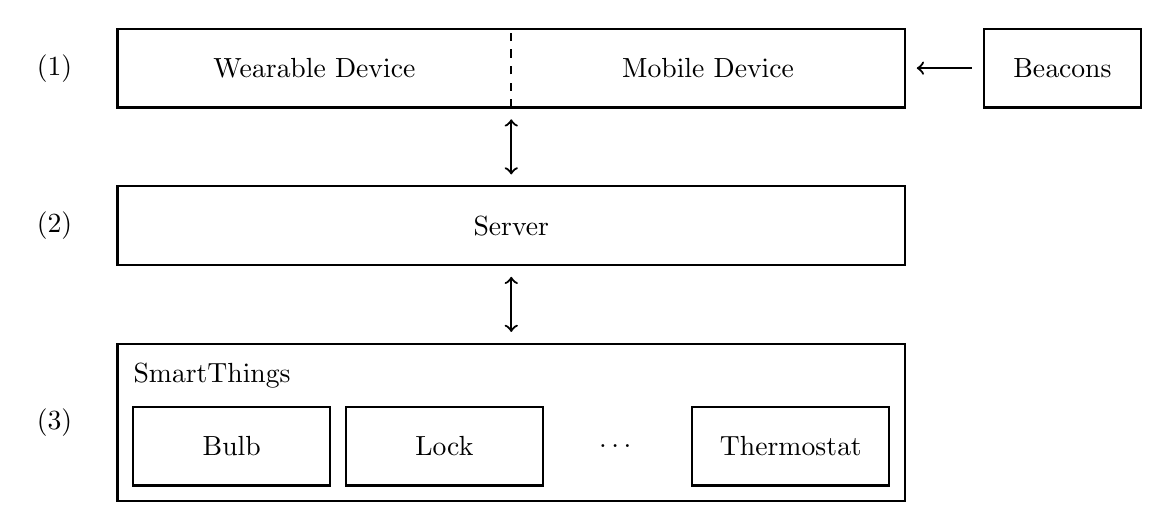
\begin{tikzpicture}
    \node[anchor=center] at (-0.8,0.5) {(1)};
    \node[anchor=center] at (-0.8,-1.5) {(2)};
    \node[anchor=center] at (-0.8,-4) {(3)};
    
    \node[anchor=center] at (2.5,0.5) {Wearable Device};
    \node[anchor=center] at (7.5,0.5) {Mobile Device};
    \draw[thick] (0,0) rectangle (10,1);
    \draw[thick, dashed] (5,0) -- (5,1);
    \draw[thick,->] (10.85,0.5) -- (10.15,0.5);
    \draw[thick] (11,0) rectangle (13,1) node[pos=.5] {Beacons};
    
    \draw[thick] (0,-1) rectangle (10,-2) node[pos=.5] {Server};
    \draw[thick,<->] (5,-0.15) -- (5,-0.85);
    
    \node[anchor=center] at (1.2,-3.4) {SmartThings};
    \draw[thick] (0,-3) rectangle (10,-5);
    \draw[thick,<->] (5,-2.15) -- (5,-2.85);
    \draw[thick] (0.2,-3.8) rectangle (2.7,-4.8) node[pos=.5] (bulb) {Bulb};
    \draw[thick] (2.9,-3.8) rectangle (5.4,-4.8) node[pos=.5] (lock) {Lock};
    \draw[thick] (7.3,-3.8) rectangle (9.8,-4.8) node[pos=.5] (door) {Thermostat};
    \node at ($(lock)!.5!(door)$) {\ldots};
\end{tikzpicture}}
\end{figure}
\end{frame}

% HomePort
% \begin{frame}{Architecture}{HomePort}
% \centering
% \begin{figure}
%   \subfloat{
%     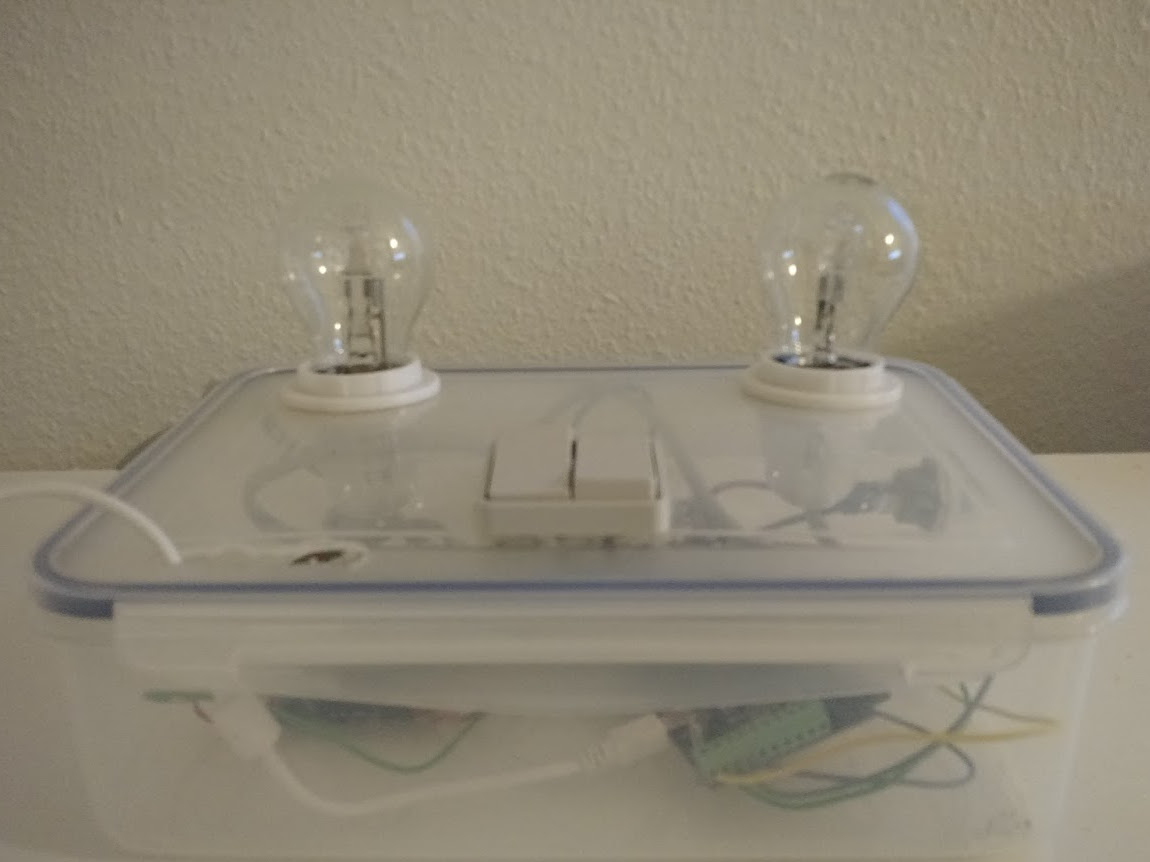
\includegraphics[width=0.48\textwidth]{../images/phidget_off}
%   }
%   \subfloat{
%     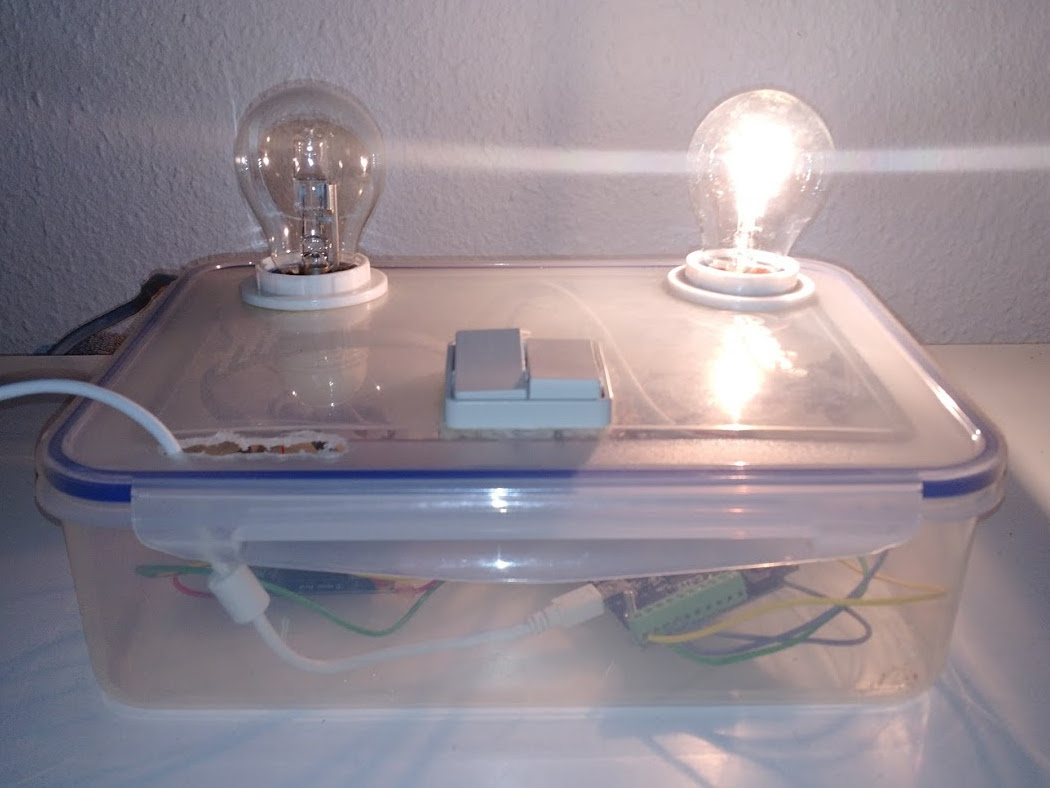
\includegraphics[width=0.48\textwidth]{../images/phidget_on}
%   }
% \end{figure}
% \end{frame}

%%% Local Variables:
%%% mode: latex
%%% TeX-master: "../AAUsimpletheme"
%%% End:


\begin{frame}{Gesture Recognition}{}
\centering
\begin{figure}
    \subfloat{
        \frame{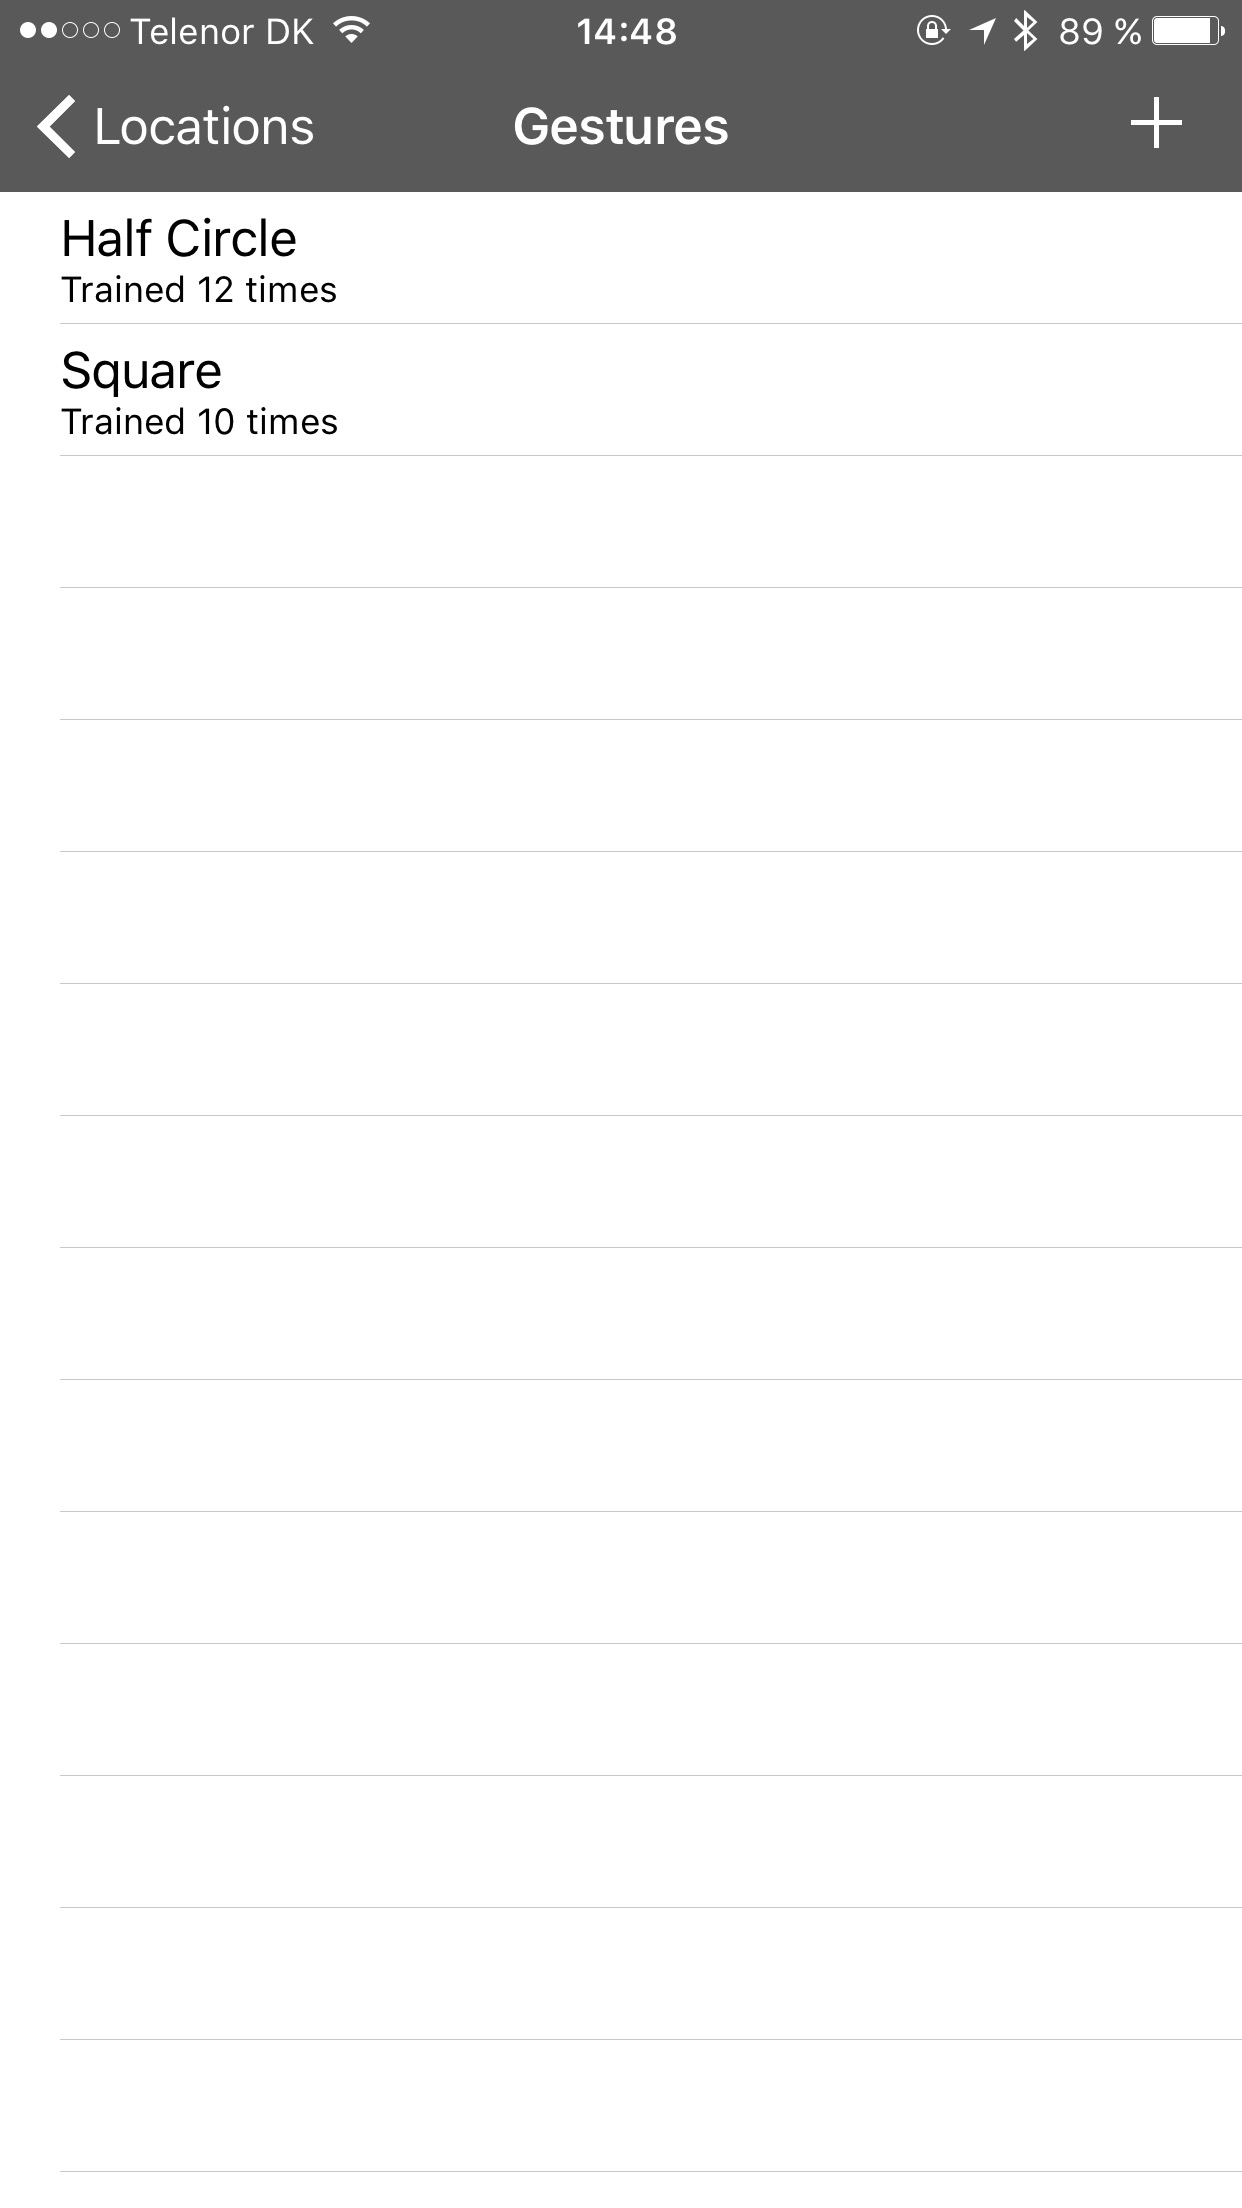
\includegraphics[width=0.3\textwidth]{../images/prototype-3-all-gestures}}
    }
    \subfloat{
        \frame{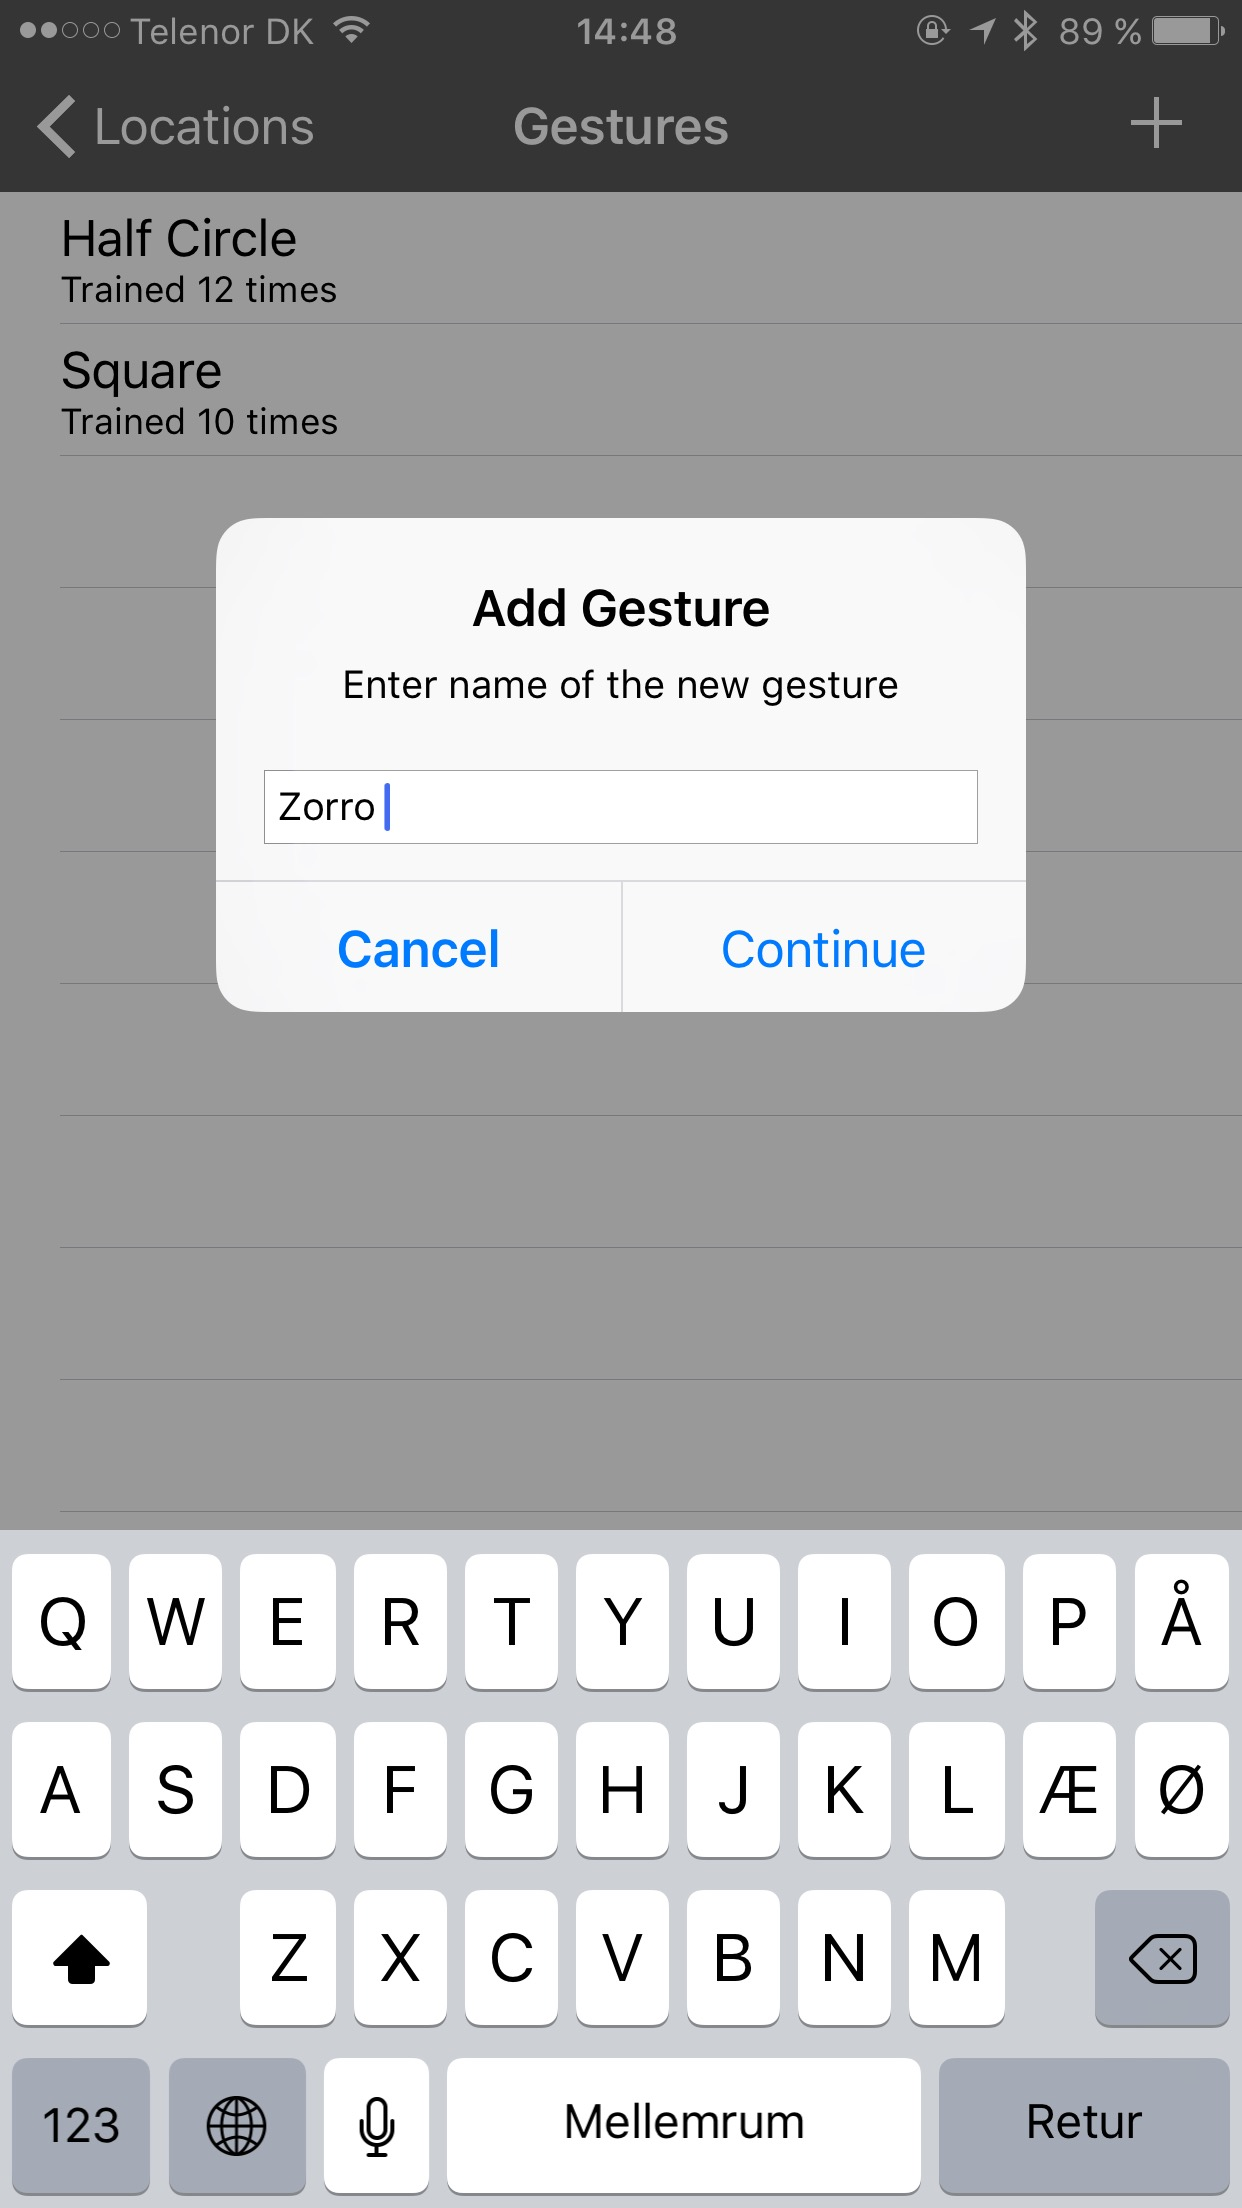
\includegraphics[width=0.3\textwidth]{../images/prototype-3-new-gesture}}
    }
    \subfloat{
        \frame{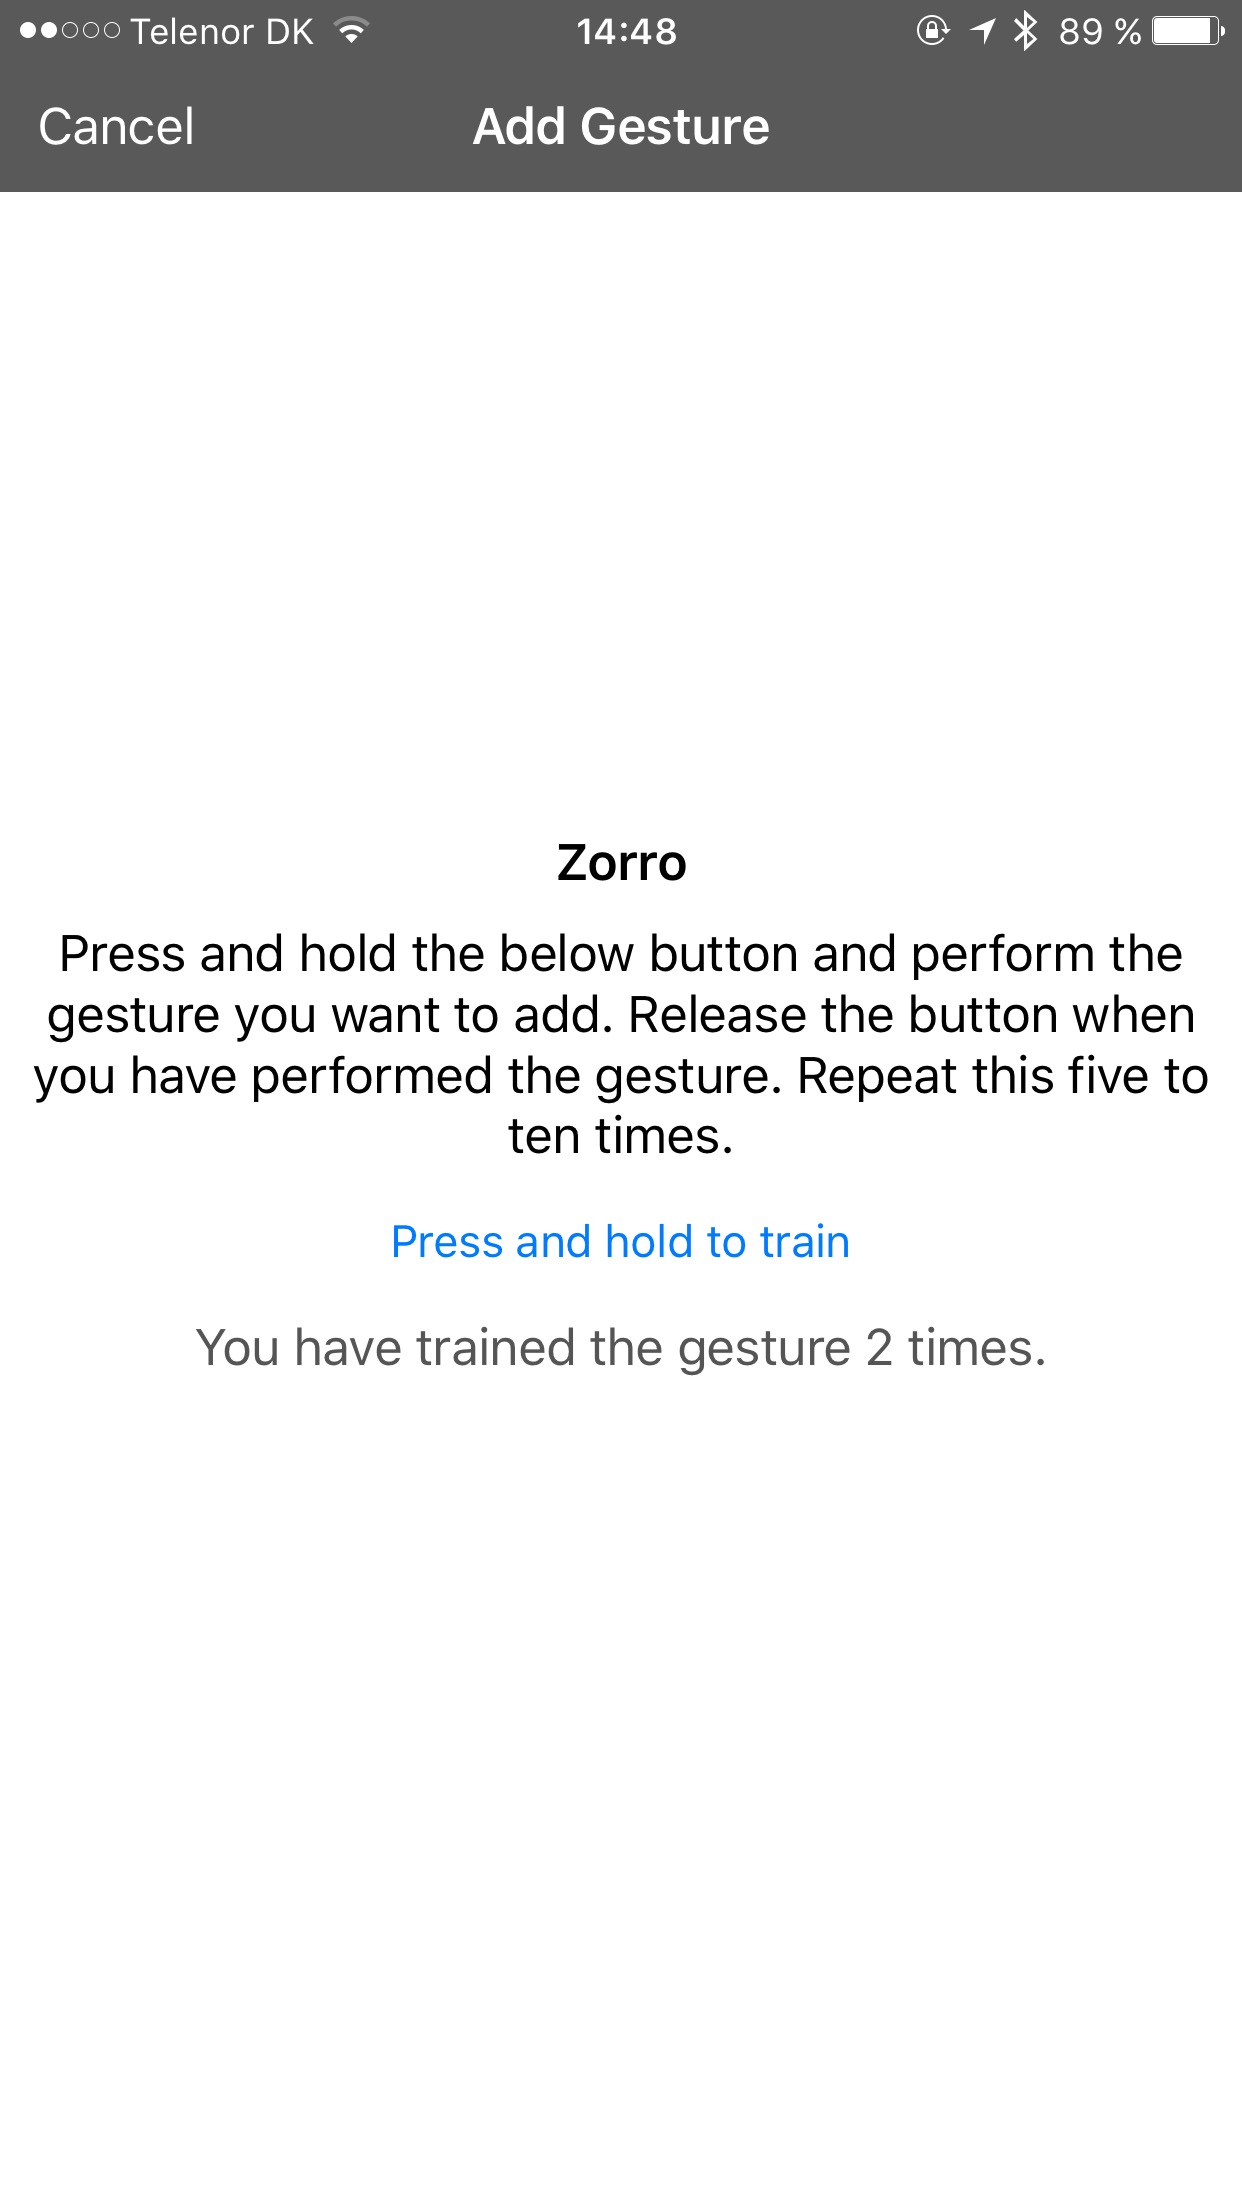
\includegraphics[width=0.3\textwidth]{../images/prototype-3-train-gesture}}
    }
\label{fig:prototype3-gesture-screenshots}
\end{figure}
\end{frame}

\begin{frame}{Gesture Recognition}{Point Detection}
\centering
\begin{figure}
    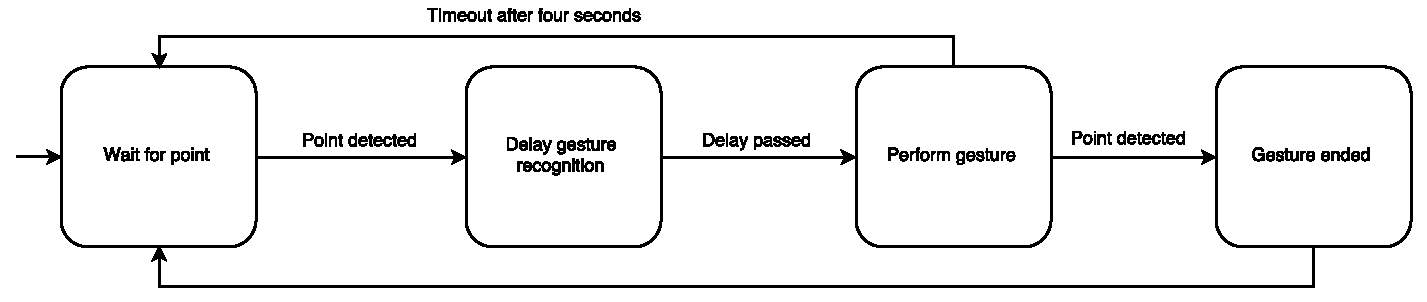
\includegraphics[width=\textwidth]{../images/point-to-gesture-state-diagram}
\label{fig:point-to-gesture-state-diagram}
\end{figure}
\end{frame}
\section{Orientation}\label{sec:analysis:orientation}
In this project, a solution for pointing at a controllable device, \eg a lamp, is proposed. 
In order to determine which device the user points at, 
and thereby intends to control, 
it is necessary to determine the locations of the devices in the system, 
relative to the user. 
Thus we must know the location of the user, 
and his controllable devices along with the orientation of the user.

The orientation of the user can be retrieved from any device possessing a magnetometer. 
We found that \num{49} devices in Vandrico's database contain the magnetometer component, 28 of which are worn on the wrist.
With a total of 163 wearables worn on the wrist, that means only 17\% of the wearables worn on the wrist has a magnometer. However, alternatives to the magnometer requires the user to install extra hardware in is home. This is the case with the infared technology utilized by Reemo.

We also need to define a visibility range, 
\ie a range that constitutes the area in which items are visible to the system. 
This range can be specified (in degrees) as $r = o \pm e$, 
where $r$ is the visibility range, $o$ is the orientation of the user, 
and $e$ is the distance between $o$ and the edges of $r$.
\Cref{fig:visibilityangle} illustrates the visibility angle. 
In \Cref{fig:visibilityangle}, the user's orientation is \var{o1}, 
and there are two devices with orientations \var{o2} and \var{o3}. 
An orientation in degrees is between \num{0} and \num{360}. 
To determine whether a device with orientation \var{o2} is within the visibility range, 
it is a simple matter of calculating whether \var{o2} is greater than $\var{o1}-\var{e}$, 
and smaller than $\var{o1}+\var{e}$, 
with some exceptions when the visibility range spans the gap between 359\degree \ and 0\degree.

Given the user's location $(x1, y1)$ and the devices locations $(x2, y2)$ and $(x3, y3)$,
we can calculate the angle between the devices' orientation (\var{o2} and \var{o3}), 
by finding the inverse tangent (arctangent), 
and then converting from radians to degrees (dividing \num{180} by $\pi$), 
such that we get the following equation:

\begin{equation}\label{eq:angle}
\var{angle} = 180 / \pi * \arctan((\var{user.y} - \var{device.y}) / (\var{user.x} - \var{device.x}))
\end{equation}

\begin{figure}[!htb]
    \centering
    \def\svgwidth{0.6\textwidth}
    \import{drawings/}{drawings/visibilityangle.pdf_tex}
    \caption{Finding objects in the visibility range. Device 1 is within the range, but Device 2 is not.}
\label{fig:visibilityangle}
\end{figure}

%%% Local Variables:
%%% mode: latex
%%% TeX-master: "../../master"
%%% End:

\section{Indoor Positioning}

\begin{frame}{Locating the user}{}
\centering
\begin{figure}[!htb]%
    \frame{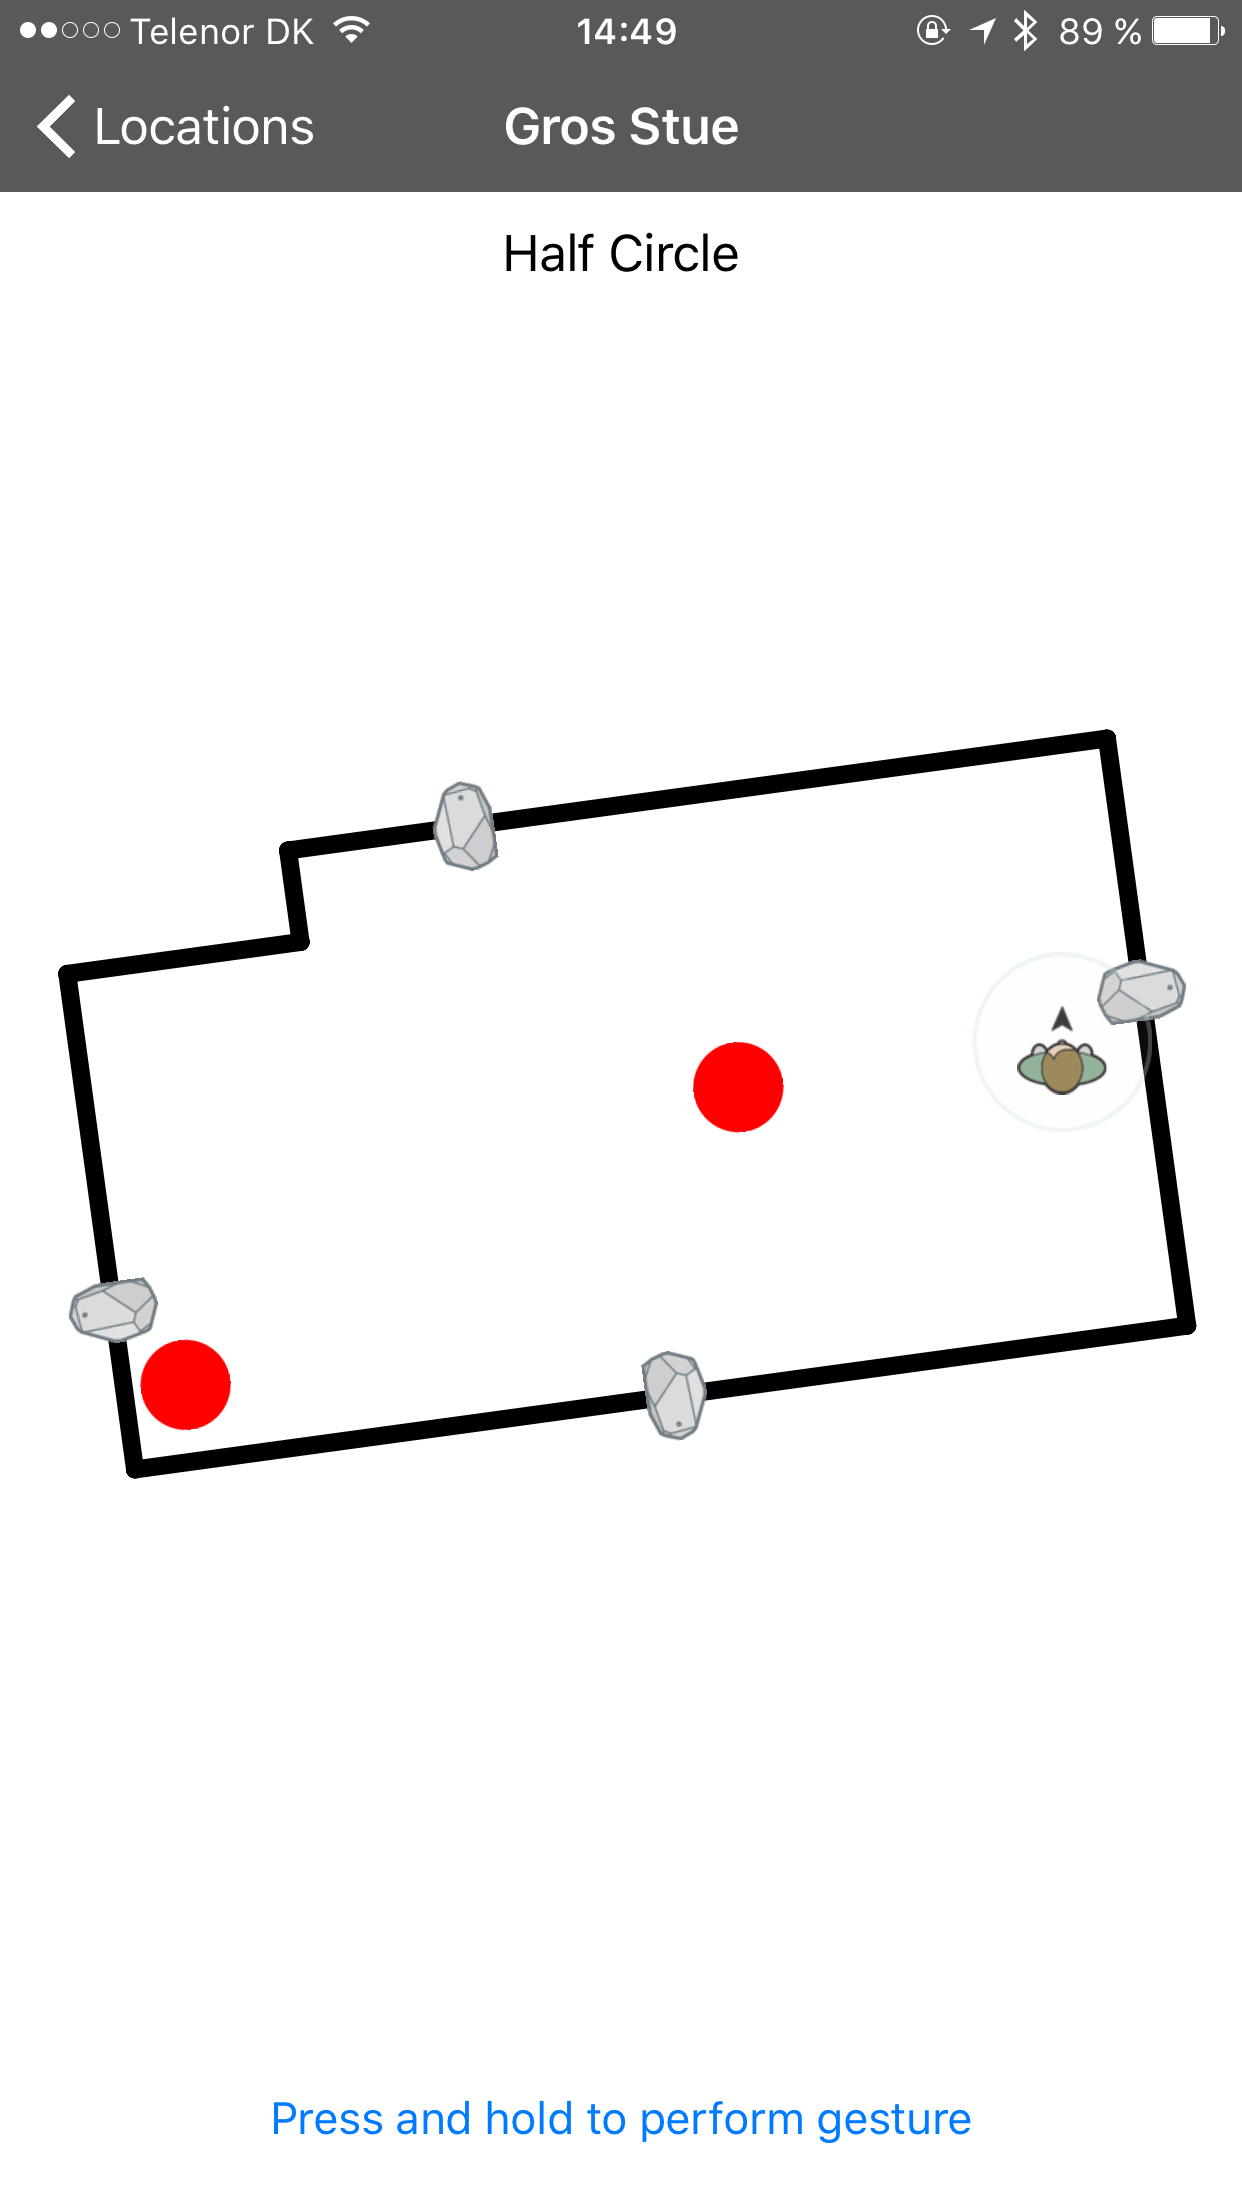
\includegraphics[width=0.3\textwidth]{../images/prototype-3-gesture-triggered}}
\label{fig:prototype3-room-screenshot}
\end{figure}
\end{frame}

\begin{frame}{Locating the user}{}
\begin{figure}[!htb]
  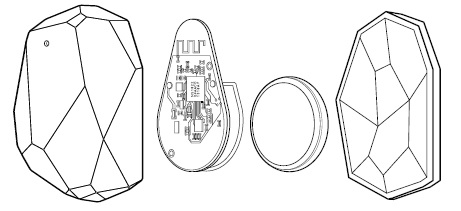
\includegraphics[width=0.6\textwidth]{../images/estimotebeacon}
  \caption{Image of an Estimote beacon. Source: \protect\url{http://blog.estimote.com/post/106913675010/how-do-beacons-work-the-physics-of-beacon-tech}.}
  \label{fig:estimotebeacon}
\end{figure}
\end{frame}

\chapter{Evaluation}\label{chap:evaluation}
This chapter describes the tests and experiments we setup in order to evaluate our solution. 
We setup \num{4} tests, one in each of the following sections. 
The first test, described in \Cref{sec:gestureperformance}, we perform, 
is to measure the performance of the gesture recognizer described in \Cref{sec:gesturerecognition}. 
Then we evaluate the correctness of the gesture recognizer in \Cref{sec:gesturecorrectness}.
To test the precision of our indoor location, 
we perform precision tests on the Estimote SDK in \Cref{sec:estimoteprecision}.
Being able to detect points, and thus when to start recognizing gestures, we implemented a point detector. This detector is evaluated in \Cref{sec:evaluation:pointing}.
The server and the smart hub, HomePort, is briefly evaluated in \Cref{sec:servereval}.
Finally we test the system as a whole in \Cref{sec:evaluation:system-correctness}.

\section{Performance of Gesture Recognition}
Gesture recognition is a core part of our solution and it is being performed often. 
Since the gesture recognition is being performed by device with somewhat low performance,
it is important that we have high performance of our gesture recognition. 
In this section we test the performance of recognizing gestures. 
We test the performance by executing a number of gestures and see how fast we can recognize these.  
We expect the number of unique gestures in the database to increase the recognition time. 
Furthermore, the number of times each gesture has been trained also increase the complexity of recognizing gestures. %Thalley: Remove this line if that is no longer the case

For this setup, we have [NUMBER OF GESTURES], each trained [NUMBER OF TRAININGS] times. 
We start by evaluating with \num{1} gesture, and then increase the number of unique gestures to estimate the computational complexity.

\begin{figure}[!htb]
    \centering
    \todo[author=Thalley]{Insert figure}
    \caption{Graph showing the time of recognizing gestures, with increasing number of unique gestures}
    \label{fig:performancegraph}
\end{figure}
\todo[author=Thalley]{Perform performance of gesture recognition tests}

The result from \Cref{fig:performancegraph} show that the complexity of gesture recognition is [RESULT]. 

To find the time it takes to recognize a single gesture, 
we perform the recognition of a random sample of known gestures \num{1000} times, 
and calculate the mean time spend on recognizing each gesture. 
Since the number of unique gestures has an impact on the complexity, 
we choose a fixed number of common gestures each trained [NUMBER OF TRAININGS] times. 
We expect at common number of unique gestures to be [NUMBER OF COMMON GESTURES], 
and for that number of gestures we find that the average time to recognize a single gesture is [RESULT]. 

\subsection{Performance of Gesture Recognition Conclusion}
From the results, we can conclude that... \todo[author=Thalley]{Write conclusion of performance test based on results}

\section{Correctness Rate of Gesture Recognition}\label{sec:gesturecorrectness}
%Thalley: if this changes, make sure to change this section
%Thalley: If we want to perform our own tests based on e.g. the gestures in previous section, rewrite this
We are using the \$3 Gesture Recognizer and they have in their paper, 
presenting the recognition system, performed this test \cite{threedollar}.
They had \num{12} volunteers testing the system with a Nintendo Wii remote, 
on a set of \num{8} unique gestures (defined in their paper).
They post a result of a correctness rate of \perc{80}. 
They also post a clear difference between the volunteers, 
where the best score was a correctness rate of \perc{98} and the worst score was \perc{58}. 
\subsection{Correctness Rate of Gesture Recognition Conclusion}
From the results, we can conclude that the \$3 Gesture Recognizer is adequate for this project, but leaves room for improvement. 
\todo[author=Thalley]{Find and compare their results to other gesture recognizer results or results from e.g. voice recognition?} 
\section{Precision of Indoor Location}\label{sec:estimoteprecision}
Another core part of our system is indoor location. 
For the ``point-to-select'' part of our system to work as intended, 
we need high indoor precision. 
In \Cref{sec:designindoorlocation} we mentioned that Estimote claims the accuracy to be \num{0.5}-\num{1} meters.
In this section we test if that is actually the case, 
or even if we can achieve better results than that. 
This section will contain some of the measurements from our tests. 
All of the measurements can be found in \Cref{app:estimotetestresults}

We test this by comparing the position we get from the application, \ie from the Estimote beacons,
to the actual position we have measured in the room. 
We test in with the \num{4} settings from \Cref{table:rooms}.

\begin{table}
  \centering
  \begin{tabular}{l| l c c c}
    Name & Size in meters & \# of Beacons & \# of Tests & \# of WiFi Access Points\\ \hline
    Room 1 & $5 \times 5$ & 4 & 8 & 19 \\
    Room 2 & $8 \times 8$ & 4 & 7 & 19 \\
    Room 3 & $17.9 \times 17.9$ & 4 & 3 & 3\\
    Room 4 & $4.9 \times 9.95$ & 4/8 & 33 & 20 
  \end{tabular}
  \caption{Room settings}
  \label{table:rooms}
\end{table}

We test in different settings to measure if, and how much, 
the size of the room matters in terms of accuracy. 
We decided to test outside in an area where there were none or few WiFi signals,
as WiFi shares the same same radio frequency as BLE (\SI{2.4}{\GHz}). 
We have performed tests both with and without movement. 
The same person performed all the movement tests. 

\subsection{Setup}\label{sec:setup}
Room 1 and Room 2 were setup in an auditorium. 
We used tables to simulate walls, 
and we placed the beacons on chairs on top of the tables. 
The setup can be seen in \Cref{fig:audtest} and illustrated in \Cref{fig:precisiontest:illustration}. 
\begin{figure}[!htb]
  \centering
  \includegraphics[width=\textwidth]{drawings/audtest}
  \caption{The setup for Room 1 and Room 2. Room 1 is marked as the inner (blue) square and is $5 \times 5$ meters. Room 2 is marked as the outer (red) square and is $8 \times 8$ meters. The Estimote beacons are placed on the chairs.}
  \label{fig:audtest}
\end{figure}

\begin{figure}[!htb]
  \centering
  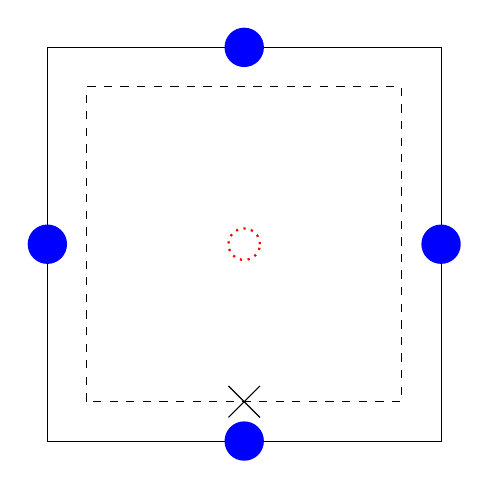
\begin{tikzpicture}

\draw (0,0) rectangle (5,5); % Outline of room

\draw[red,thick,dotted] (2.5,2.5) circle (0.2); % Phone location

\fill[blue!100!] (2.5, 0) circle (0.25); % Beacon location - Bottom
\fill[blue!100!] (5, 2.5) circle (0.25); % Beacon location - Right
\fill[blue!100!] (2.5, 5) circle (0.25); % Beacon location - Top
\fill[blue!100!] (0, 2.5) circle (0.25); % Beacon location - Left

% Walking path
\draw[dashed] (0.5,0.5) rectangle (4.5,4.5);

% Start / stop point of walking path
\draw (2.3,0.7) -- (2.7,0.3);
\draw (2.3,0.3) -- (2.7,0.7);

\end{tikzpicture}
  \caption{Illustration of room used for indoor location precision test. The full (blue) circles represent beacons, the dotted line is the walking path (movement test) and the dotted center circle is the location of the phone (stationary test).}
  \label{fig:precisiontest:illustration}
\end{figure}

The setup consisted of four beacons, one on each wall, 
each recommended settings from Estimote \cite{estimote:settings}:
\begin{description}
  \item[Broadcasting Power:]{\num{4} dBm}
  \item[Advertising Interval:]{\SI{200}{\milli\second}}
  \item[Smart Power Mode:]{Enabled}
  \item[Basic Power Mode:]{Disabled}
\end{description}
The beacons run firmware version A3.2.0 and hardware version,
and the broadcasting scheme is the Estimote default scheme (\ie). 

For Room 3, the outdoor ``room'',
we attached the beacons to lampposts. 
We tested outside to see if the number of access points would have, and how much of, 
an impact on the accuracy. 
The ``room'' is illustrated in \Cref{fig:outdoortest}. 
The beacons in this room are slightly off-center (\SI{0.45}{\meter}), 
as we had to use the lampposts' locations. 

\begin{figure}[!htb]
  \centering
  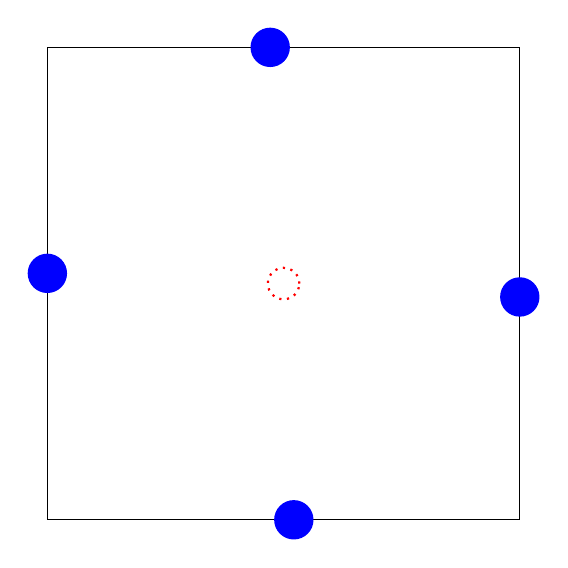
\begin{tikzpicture}

\draw (0,0) rectangle (6,6); % Outline of room
%
\draw[red,thick,dotted] (3,3) circle (0.2); % Phone location

\fill[blue!100!] (3.13, 0) circle (0.25); % Beacon location - Bottom
\fill[blue!100!] (6, 2.83) circle (0.25); % Beacon location - Right
\fill[blue!100!] (2.83, 6) circle (0.25); % Beacon location - Top
\fill[blue!100!] (0, 3.13) circle (0.25); % Beacon location - Left

\end{tikzpicture}
  \caption{Illustration of room used for Estimote accuracy outdoors, with little to no interference from WiFi access points. The full (blue) circles represent beacons, and the dotted center circle is the location of the phone (stationary test).}
  \label{fig:outdoortest}
\end{figure}

Room 4 is a seminar room. 
The setup for Room 4 for the stationary tests,
were exactly the same as the Room 1 and 2. 
We also did movement tests in this room, 
where the user walked around near the walls as with Room 1 and 2. 
We did, however, also test movement where the user walked in a \emph{bowtie},
illustrated by \Cref{fig:bowtie4beacons}. 
We did this to see if we it would have any effect if we did not walk near the beacons all the time. 
We also tried to perform tests with \num{8} beacons in this room, 
illustrated by \Cref{fig:bowtie8beacons}. 

\begin{figure}[!htb]
  \begin{minipage}[b]{0.45\textwidth}
    \centering
    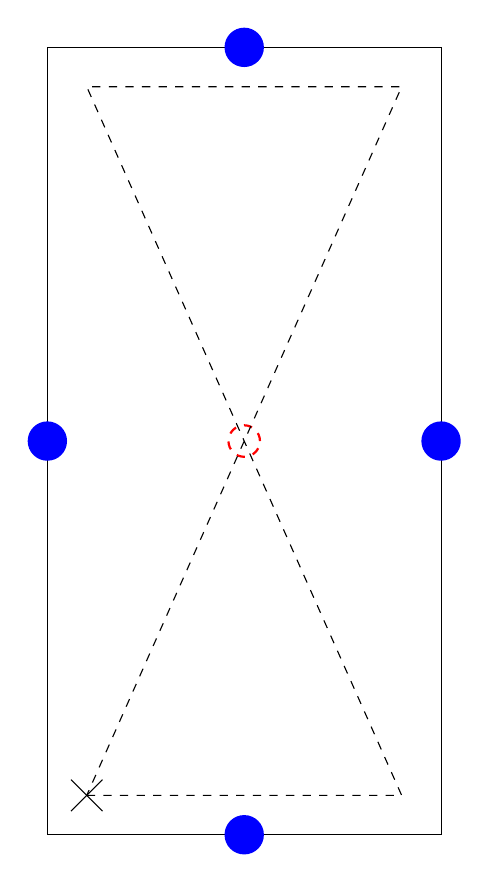
\begin{tikzpicture}

\draw (0,0) rectangle (5,10); % Outline of room

\draw[red,thick,dashed] (2.5,5) circle (0.2); % Phone location

\fill[blue!100!] (2.5, 0) circle (0.25); % Beacon location - Bottom
\fill[blue!100!] (5, 5) circle (0.25); % Beacon location - Right
\fill[blue!100!] (2.5, 10) circle (0.25); % Beacon location - Top
\fill[blue!100!] (0, 5) circle (0.25); % Beacon location - Left

% Walking path
\draw[dashed] (0.5,0.5) -- (4.5,0.5) -- (0.5, 9.5) -- (4.5, 9.5) -- cycle;

% Start / stop point of walking path
\draw (0.3,0.7) -- (0.7,0.3);
\draw (0.3,0.3) -- (0.7,0.7);

\end{tikzpicture}
    \caption{Room 4 bowtie setup using four beacons.}
    \label{fig:bowtie4beacons}
  \end{minipage}\hfill
  \begin{minipage}[b]{0.45\textwidth}
    \centering
    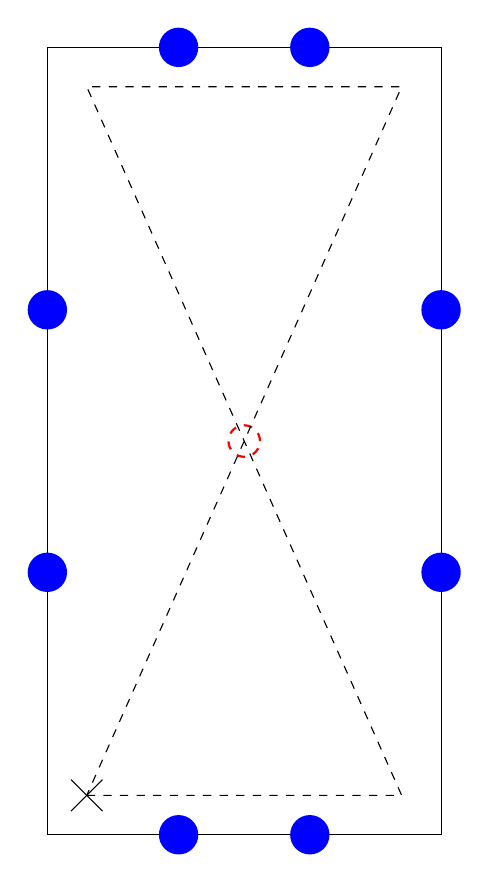
\begin{tikzpicture}

\draw (0,0) rectangle (5,10); % Outline of room

\draw[red,thick,dashed] (2.5,5) circle (0.2); % Phone location

\fill[blue!100!] (1.6667, 0) circle (0.25); % Beacon location - Bottom Left
\fill[blue!100!] (3.3334, 0) circle (0.25); % Beacon location - Bottom Right
\fill[blue!100!] (5, 6.6666) circle (0.25); % Beacon location - Right Top
\fill[blue!100!] (5, 3.3333) circle (0.25); % Beacon location - Right Bottom
\fill[blue!100!] (1.6667, 10) circle (0.25); % Beacon location - Top Left
\fill[blue!100!] (3.3334, 10) circle (0.25); % Beacon location - Top Right
\fill[blue!100!] (0, 6.6666) circle (0.25); % Beacon location - Left Top
\fill[blue!100!] (0, 3.3333) circle (0.25); % Beacon location - Left Bottom


% Walking path
\draw[dashed] (0.5,0.5) -- (4.5,0.5) -- (0.5, 9.5) -- (4.5, 9.5) -- cycle;

% Start / stop point of walking path
\draw (0.3,0.7) -- (0.7,0.3);
\draw (0.3,0.3) -- (0.7,0.7);

\end{tikzpicture}
    \caption{Room 4 bowtie setup using eight beacons.}
    \label{fig:bowtie8beacons}
  \end{minipage}
\end{figure}

\Cref{table:precisiontest:roomsize} shows the test setups from these rooms.
In \Cref{sec:settings}, we change some of the settings to determine if they have any effect.

\begin{table}[!htb]
  \centering
  \begin{tabular}{l| l l c c}
    Room   & Phone Position & Duration 	       & Test Count & \# of Beacons \\ \hline
    Room 1 & Center         & \SI{1}{\minute}  & 4          & 4 \\ 
    Room 1 & Center         & \SI{2}{\minute}  & 1          & 4 \\ 
    Room 1 & Moving         & NA               & 3          & 4 \\
    Room 2 & Center         & \SI{1}{\minute}  & 3          & 4 \\ 
    Room 2 & Center         & \SI{2}{\minute}  & 1          & 4 \\
    Room 2 & Moving         & NA               & 3          & 4 \\ 
    Room 3 & Center         & \SI{1}{\minute}  & 3          & 4 \\ 
    Room 4 & Center         & \SI{1}{\minute}  & 3          & 4 \\ 
    Room 4 & Center         & \SI{1}{\minute}  & 3          & 8 \\ 
    Room 4 & Moving         & NA               & 3          & 4 \\
    Room 4 & Moving         & NA               & 3          & 8 \\
    Room 4 & Moving-Bowtie  & NA               & 3          & 4 \\
    Room 4 & Moving-Bowtie  & NA               & 3          & 8 \\
  \end{tabular}
  \caption{Tests conducted with varying room size and recommended beacon configuration.}
  \label{table:precisiontest:roomsize}
\end{table}

\subsection{Stationary Accuracy}
This section contains the results from measuring the accuracy of the tests, 
where we have placed a phone and logged the locations. 
\Cref{fig:room3:1:4:c,fig:room4:1:4:c,fig:room4:1:4:2.8,fig:room4:1:8:c} shows selected results as heatmaps. 
In these heatmaps, the heat, or intensity, 
shows the number of coordinates measured at that coordinate. 
Located the to the right of each of these figures, 
is a graph showing the distance error from that test. 
We use the Euclidean distance to calculate the distance error between the phone's location, 
and the each of the locations reported by the app:
\begin{equation}
 \var{distanceError(phone, app)} = \sqrt{(\var{phone.x} - \var{app.x})^2 + (\var{phone.y} - \var{app.y})^2}
\end{equation}

%HEATMAPS AND MEAN ERRORS
\newcommand{\graphspace}{\vspace{0.08cm}}
\begin{figure}[!htb]
  \begin{minipage}[b]{0.5\textwidth}
    \centering
    \includegraphics{\heatmap{32}}
    \graphspace
    \caption{Room 3, \SI{1}{\minute}, 4 beacons, centered}
    \label{fig:room3:1:4:c}
  \end{minipage}\hfill
  \begin{minipage}[b]{0.45\textwidth}
%    \centering
    \meanerror{32-outside-1218-1790x1790-1min.csv}{11}
    \caption{Distance error from \Cref{fig:room3:1:4:c}}
    \label{fig:distance:room3:1:4:c}
  \end{minipage}
\end{figure}

\begin{figure}[!htb]
  \begin{minipage}[b]{0.5\textwidth}
    \centering
    \includegraphics{\heatmap{36}}
    \graphspace
    \caption{Room 4, \SI{1}{\minute}, 4 beacons, centered}
    \label{fig:room4:1:4:c}
  \end{minipage}\hfill
  \begin{minipage}[b]{0.45\textwidth}
    \centering
    \meanerror{36-1911-1027-490x995-1min.csv}{4}
    \caption{Distance error from \Cref{fig:room4:1:4:c}}
    \label{fig:distance:room4:1:4:c}
  \end{minipage}
\end{figure}

\begin{figure}[!htb]
  \begin{minipage}[b]{0.5\textwidth}
    \centering
    \includegraphics{\heatmap{43}}
    \graphspace
    \caption{Room 4, \SI{1}{\minute}, 4 beacons, at (2,8)}
    \label{fig:room4:1:4:2.8}
  \end{minipage}\hfill
  \begin{minipage}[b]{0.45\textwidth}
    \centering
    \meanerror{43-1911-1106-490x995-1min-at-8.2.csv}{3}
    \caption{Distance error from \Cref{fig:room4:1:4:2.8}}
    \label{fig:distance:room4:1:4:2.8}
  \end{minipage}
\end{figure}

\begin{figure}[!htb]
  \begin{minipage}[b]{0.5\textwidth}
    \centering
    \includegraphics{\heatmap{51}}
    \graphspace
    \caption{Room 4, \SI{1}{\minute}, 8 beacons, centered}
    \label{fig:room4:1:8:c}
  \end{minipage}\hfill
  \begin{minipage}[b]{0.45\textwidth}
    \centering
    \meanerror{51-1911-1137-490x995-1min-8-beacons.csv}{4}
    \caption{Distance error from \Cref{fig:room4:1:8:c}}
    \label{fig:distance:room4:1:8:c}
  \end{minipage}
\end{figure}

The heatmaps shows that none of the results are very accurate. 
However, we do see some consistency in the data, in the form of clusters. 
This is primary seen in \Cref{fig:room3:1:4:c,fig:room4:1:4:2.8}. 
We do see some clustering in \Cref{fig:room4:1:4:c}. 
We expect the reason why the data is spread out like that, 
is a combination of the fact that the phone is centered, \ie not near any beacons,
and that we are near WiFi access points with the same frequency. 
We see a similar tendency in in \Cref{fig:room4:1:8:c}, 
but we expect that the increased spreading here is due to interference from using more beacons. 

The distance error graphs supports the statement that none of the results are very accurate. 
It is clearly worst in the outside test, shown by \Cref{fig:distance:room3:1:4:c}. 
\Cref{fig:distance:room4:1:4:2.8,fig:distance:room4:1:4:c} show some decent results. 
\Cref{fig:distance:room4:1:4:2.8}, where the phone is not centered, 
is clearly the best result we get. 
An interesting result is seen by \Cref{fig:room4:1:8:c},
where it seems that the number of beacons, 
makes the measurements fluctuate. 

\Cref{table:meanerrorresults} shows the \emph{mean} distance error of all the stationary tests. 

\begin{table}[!htb]
  \centering
  \begin{tabular}{l|l c c}
    Room   & Position   & \# of beacons & Mean error \\ \hline
    Room 1 & Centered   & 4             & \SI{1.78}{\meter} \\
    Room 2 & Centered   & 4             & \SI{2.96}{\meter} \\
    Room 3 & Centered   & 4             & \SI{7.31}{\meter} \\
    Room 4 & Centered   & 4             & \SI{1.94}{\meter} \\
    Room 4 & At $(2,8)$ & 4             & \SI{1.22}{\meter} \\
    Room 4 & Centered   & 8             & \SI{3.02}{\meter} \\ \hline
    Total  &            &               & \SI{2.92}{\meter}
  \end{tabular}
  \caption{Mean error of all stationary tests with Estimote recommended settings. Some rooms have more test results than others. See \Cref{table:rooms}.}
  \label{table:meanerrorresults}
\end{table}

Based on this table, we can conclude the following:
\begin{itemize}
  \item The distance error increases as we increase the distance to the beacons
  \item Adding more beacons results in worse accuracy
\end{itemize}

Increasing the distance to the beacons, results in weaker signals from the beacons. 
It is thus expectable that the accuracy is worse further away from the beacons. 

Regarding the worse accuracy with more beacons, 
we have two theories to why.
The first theory is that the Estimote SDK only uses a subset of beacons, \eg only \num{4}, for accuracy. 
The reasoning behind this theory is that in \Cref{fig:distance:room4:1:8:c}, 
we consistent change between \SI{3.5}{\meter} and \SI{2.5}{\meter}, 
where from the tests with \num{4} (\Cref{fig:distance:room3:1:4:c,fig:distance:room4:1:4:c,fig:distance:room3:1:4:2.8}) beacons, 
we see a convergence after the first \num{50} measurements.
The change could be a result of the Estimote changing from two sets of \num{4} beacons, 
where the \SI{3.5}{\meter} results are from one set, 
and the \SI{2.5}{\meter} results are from the other set. 
Estimote has not provided any documentation about how many beacons is used to get the location using the SDK, 
nor are we able to see this from the SDK. 

The other theory is that the beacons interfere with each other. 
With \num{8} beacons in a $5 \times 10$ meter room, 
it is possible that the signals interfere with each other, 
when the beacons are placed near to each other. 
In Estimote's guide for beacon placement \cite{SIGNALBLEED}, 
they write:
\begin{quote}
  ``If you’re using many beacon regions in close proximity to each other, it’s likely that you will experience \emph{signal bleed}: beacons from one region being detected in the other.''
\end{quote}
So it is possible that the signals we read from a beacon is from another beacon,
and thus we get a wrong reading.  

\FloatBarrier
\subsection{Moving Accuracy}
In this section we measure the accuracy of the Estimote beacons,
while the phone is in motion. 
We walk around in a given path, 
as described by \Cref{sec:setup}.
\Cref{fig:room1:4:m,fig:room2:4:m,fig:room4:4:m} shows selected heatmaps of walking near the walls, 
where \Cref{fig:room4:4:b,fig:room4:8:b} shows selected heatmaps of walking in a bowtie pattern.
%HEATMAPS
\begin{figure}[!htb]
  \begin{minipage}{0.48\textwidth}
    \centering
    \includegraphics[width=\textwidth]{\heatmap{08}}
    \caption{Room 1, 4 beacons, moving}
    \label{fig:room1:4:m}
  \end{minipage}\hfill
  \begin{minipage}{0.48\textwidth}
    \centering
    \includegraphics[width=\textwidth]{\heatmap{14}}
    \caption{Room 2, 4 beacons, moving}
    \label{fig:room2:4:m}
  \end{minipage}
\end{figure}
\begin{figure}[!htb]
  \centering
  \includegraphics[width=0.48\textwidth]{\heatmap{37}}
  \caption{Room 4, 4 beacons, moving}
  \label{fig:room4:4:m}
\end{figure}

\Cref{fig:room1:4:m,fig:room2:4:m} shows that the coordinates we get, 
were relatively close to where we walked, 
but had trouble near the corners, \ie further away from the beacons. 
\Cref{fig:room4:4:m} shows poor results. 
The main difference between rooms 1 and 2 and Room 4,
besides the size,  
is that Room 4 has actual walls, 
instead of the simulated walls. 
As walls can bounce radio waves from the beacons,
this is likely the reason why the results from Room 4 are worse. 

\begin{figure}[!htb]
  \begin{minipage}{0.48\textwidth}
    \centering
    \includegraphics[width=\textwidth]{\heatmap{40}}
    \caption{Room 4, 4 beacons, bowtie}
    \label{fig:room4:4:b}
  \end{minipage}\hfill
  \begin{minipage}{0.48\textwidth}
    \centering
    \includegraphics[width=\textwidth]{\heatmap{48}}
    \caption{Room 2, 8 beacons, bowtie}
    \label{fig:room4:8:b}
  \end{minipage}
\end{figure}
Like with \Cref{fig:room4:4:m}, \Cref{fig:room4:4:b,fig:room4:8:b} show poor results. 
This is likely due to walls, as with before, 
but also that we are now spending more time walking further away from beacons, 
than we did in \Cref{fig:room1:4:m,fig:room2:4:m}.

\subsection{Changing Settings}\label{sec:settings}
For this test the objective was to test the accuracy of the location system,
using different settings. 
We use Room 4 with 4 beacons for these tests. 
The tests conducted in this room, 
had the phone placed on a table in the center of the room, 
and logging position data for a duration of one minute.
This was done three times, 
and then the settings of the beacons were changed.

The difference settings we tested are shown in \Cref{table:precisiontest:settings}.
Each result describes the mean error distance from \num{3} tests, 
each \num{1} minutes long.  

\begin{table}[!htb]
  \centering
  \begin{tabular}{c|c|c}
    Advertising Interval    & Broadcasting Power & Mean Error Distance \\ \hline
    \SI{200}{\milli\second} & \num{-20} dBm      & \SI{4.57}{\meter} \\ 
    \SI{200}{\milli\second} & \num{-12} dBm      & \SI{3.49}{\meter} \\ 
    \SI{200}{\milli\second} & \num{-4} dBm       & \SI{2.16}{\meter} \\ 
    \SI{200}{\milli\second} & \num{4} dBm        & \SI{2.81}{\meter} \\ 
    \SI{100}{\milli\second} & \num{4} dBm        & \SI{1.41}{\meter} \\ 
  \end{tabular}
  \caption{Tests conducted with varying settings on the beacons. Each result is from $3 \times 1$ minutes of measurement.}
  \label{table:precisiontest:settings}
\end{table}

The results from \Cref{table:precisiontest:settings} show that settings do have an impact on accuracy,
but they do also have an impact on battery life. 
While changing from \SI{200}{\milli\second} to \SI{100}{\milli\second} almost increased accuracy by \perc{200},
it also increases the battery usage by \perc{200}.
Lower broadcasting powers such as \num{-20} dBm and \num{-12} dBm perform bad. 
This is because at such lower powers, 
the signal from the beacons might not have reached the phone, 
and the lack of data from these beacons is very likely to have worsened the accuracy.

Interestingly, \num{-4} dBm performed better than \num{4} dBm.
From \Cref{table:meanerrorresults}, we saw that more beacons worsened the accuracy. 
It is possible that a broadcasting power of \num{4} dBm,
creates more interferences, and thus worse results, than \num{-4} dBm. 
We do not, however, have enough data to properly conclude this. 

\subsection{Precision of Indoor Location Conclusion}
From out results, we can conclude that we cannot, 
in our settings, reach high indoor accuracy using Estimote beacons. 
They claim that the accuracy is \num{0.5}-\num{1} meters, 
but our best result is \num{1.22} meter, 
and our average accuracy is \num{2.92} meters. 

No tendencies are shown across the results. 
This make it very hard, if not impossible,
to compensate for inaccurate results.  

\subsubsection{Considerations}
All of our experiments in this section have been performed on a single device.
We cannot say if using a different phone would provide the same results. 

Even though we have switched beacons between tests, 
so that we did not use the same ones every time, 
we have not tested if any of the beacons we have used are defect. 

The poor accuracy can also be from the SDK rather than the beacons. 
We have not tested whether we could obtain better results using other SDKs, 
not from Estimote. 

Since all of our tests were performed at locations with considerable large number of WiFi access points (see \Cref{table:rooms}),
the results could be affected by this. 
We did not test the locations in rooms with less access points, 
except for the outside room (Room 3), 
but where the size and settings of the room may have had too much effect on the results.
\section{Pointing}
\label{sec:evaluation:pointing}

A qualitative test of pointing with the device as described in section \ref{sec:detecting-points} was performed. We were interested in determining if we are able to determine when users point witht the device and when it lies on the table.

In order to perform the test we isolated the point detector in a small app that would show a white screen when no point was detected. When a point was detected, the app would show stop detecting points and show a green screen for five seconds and then start detecting points again.
This gave us a visual confirmation that a point was detected.

The test was performed by walking around a room, stopping up and pointing at an object. This was performed multiple times and in all cases the screen successfully turned green.

Furthermore we put the phone down on various tables inside the room. The screen remained white and thus not points were detected.

During our tests we did find the following two issues.

\begin{itemize}
\item Detecting a point felt slow. The time that passes from the user points with the device and the point is detected is too long. This could possibly be fixed by reducing the length of the sampling period but this may have an impact on the accuracy of the detector, i.e. it may detect points when the user did not intend to point.
\item When the phone lied on a table with small vibrations, it would detect a point. For example, typing on a laptop placed on a table will cause the table to make small vibrations. In this case, the detector may recognize a point. This could possibly be fixed by increasing the acceleration threshold for tables. However, this may negatively impact the accuracy of the detector when the user points.
\end{itemize}

%%% Local Variables:
%%% mode: latex
%%% TeX-master: "../../master"
%%% End:

\section{Server and HomePort}\label{sec:servereval}
We have tested the correctness of the server, 
but not the performance.
We have omitted testing the performance, 
as the number of requests send to the server i minimal. 

To test the correctness of the server, 
we simulate \num{5} devices,
and send both GET and POST requests to the server.
We send a total of \num{10000} requests (a mix of POST and GET) to the server, 
and validate the response received. 
We send both valid requests, 
\ie \texttt{GET /devices} and POST with valid ID and action,
but also invalid POST requests, \ie POST requests with invalid actions. 
Each of the \num{10000} requests returned the expected response code, 
\ie 200 for valid requests, and 400 for bad requests.
We can conclude that the server works as intended.

However, our third party smart hub, HomePort, showed problems. 
The implementation of HomePort that we use, 
is the so-called OldHomePort\footnote{\url{https://github.com/home-port/HomePort/tree/OldHomePort}}. 
We used this version as it was the only one with a Phidget adapter implemented. 
Through the development of the server, 
we found that this version of HomePort crashes up to a few times every minute when handling requests. 
Sometimes it will even disconnect the Phidget interface kit, 
and thus all the devices, at seemingly random points of time. 
We have not worked on determining the errors of OldHomePort, 
nor have we tried to debug it. 
This is primarily because it is a third-party component of our system, 
and has only been used to properly test the communication between the devices and the phone. 
\section{System Correctness}
\label{sec:evaluation:system-correctness}

In order to determine the system correctness given the inaccuracy of the indoor positioning described in section \ref{sec:estimoteprecision}, we created a simulation of the system.

The purpose of the simulation is to calculate how often the user points at the intended device given some inaccuracy of the indoor positioning.

The system is based on \textit{setups}. Each setup consists of the following parameters:

\begin{itemize}
\item \texttt{roomSize}: The size of some room.
\item \texttt{position}: A position of the user in the room.
\item \texttt{devices}: The devices available in the room.
\item \texttt{focusedDevice}: The device the user must point at.
\item \texttt{offset}: An offset applied to the users position.
\end{itemize}

For each setup, the simulation calculates the orientation the user must have in order to point at \texttt{focusedDevice}. The simulation then performs 100 tests for each setup. For each of those tests the users position is offsetted both horizontally and vertically by a total amount of \texttt{offset}. The horizontal offset, that is, the offset for $x$ is chosen as a random number between $-offset$ and $offset$. The vertical offset, that is, the offset for $y$ is then calculated as $y = \sqrt{offset^2 - x^2}$. We then ensure that $x \geq 0 \wedge x \leq roomSize.width \wedge y \geq 0 \wedge y \leq roomSize.height$.

One iteration of the test consists of multiple setups with different values for \texttt{position} and \texttt{focusedDevice}. We had three setups for each device in the system. Six devices were included resulting in a total of 18 setups.

For each of the 18 setups we perform 100 tests with different offsets of the user. In each of the 100 tests we find the set of devices the user points at given his position, his orientation and the set of six devices. If the \texttt{focusedDevice} is still in the set of devices the user points at, the test is considered to be accepted. 

The result of performing the 1800 tests is a percentage of how often the \texttt{focusedDevice} was in the set of visible devices. For example, a test result of 24\% indicates that 24\% of times the user still pointed at the desired device even though his location was offset by Estimote.

Since there are random numbers in the system, we may get slightly different results when performing a test with the exact same input values. Therefore we perform the 1800 tests 10 times and take the average accuracy.

This was performed seven times in order to see the influence of \texttt{offset}. That is, the influence of the inaccuracy of Estimote.

To sum up, there are four niveaus of tests:

\begin{enumerate}
\item A number of setups. In our case this is 18, three for each of the six devices in the system.
\item 100 tests for each of the setups. Each test randomly offsets the user position horizontallt and vertically resulting in a total offset of \texttt{offset}.
\item The set of 18 setups is then tested 10 times in order to calculate an average accuracy. This results in 18000 small tests where the users position is offsetted.
\item This is then done seven times with different values of \texttt{offset}.
\end{enumerate}

\subsection{Configuration}

Table \ref{tbl:evaluation:system-correctness:devices} shows the six devices used in the simulation of the system.

\begin{table}[!hbt]
\centering
\caption{Devices used in the simulation.}
\label{tbl:evaluation:system-correctness:devices}
\begin{tabular}{c|c}
\textbf{ID} & \textbf{Coordinate} \\
\hline 
1           & (6.5 ; 3.4)         \\
2           & (3.5 ; 3 ; 4)       \\
3           & (4 ; 1.8)           \\
4           & (2.5 ; 1.8)         \\
5           & (0.5 ; 0.5)         \\
6           & (2.5 ; 3.2)        
\end{tabular}
\end{table}

Table \ref{lst:evaluation:system-correctness:setups} shows the 18 setups tested. The set of setups was tested with the offsets shown in \ref{lst:evaluation:system-correctness:results} along with the achived accuracy when applying the offset to the users position.

The size of the room used in the setups matches a real world living room in a 80m\textsuperscript{2} appartment. Six devices are used as we found it reasonable in a living room of that size.

The positions used are arbitrary and less important when we calculate the orientation based on the users position and the position of the focused device.

\begin{table}[!hbt]
\centering
\caption{Setups used in the simulation. Device IDs references table \ref{tbl:evaluation:system-correctness:devices}.}
\label{lst:evaluation:system-correctness:setups}
\begin{tabular}{c|ccc}
\textbf{ID} & \textbf{Position} & \textbf{Focused device ID} & \textbf{Room size} \\
\hline
1           & (2 ; 2)           & 1                          & 6.9m x 5.37m       \\
2           & (3.4 ; 4.9)       & 1                          & 6.9m x 5.37m       \\
3           & (1.1 ; 3.6)       & 1                          & 6.9m x 5.37m       \\
4           & (0.5 ; 0.5)       & 2                          & 6.9m x 5.37m       \\
5           & (1.1 ; 3.3)       & 2                          & 6.9m x 5.37m       \\
6           & (5.5 ; 5.2)       & 3                          & 6.9m x 5.37m       \\
7           & (3 ; 2.9)         & 3                          & 6.9m x 5.37m       \\
8           & (1 ; 2)           & 3                          & 6.9m x 5.37m       \\
9           & (2.5 ; 2.3)       & 3                          & 6.9m x 5.37m       \\
10          & (4.4 ; 3.4)       & 4                          & 6.9m x 5.37m       \\
11          & (6 ; 1.2)         & 4                          & 6.9m x 5.37m       \\
12          & (5.8 ; 2.7)       & 4                          & 6.9m x 5.37m       \\
13          & (4.6 ; 1.4)       & 5                          & 6.9m x 5.37m       \\
14          & (2.3 ; 5.2)       & 5                          & 6.9m x 5.37m       \\
15          & (0.3 ; 0.1)       & 5                          & 6.9m x 5.37m       \\
16          & (6.2 ; 4.4)       & 6                          & 6.9m x 5.37m       \\
17          & (5.1 ; 2.7)       & 6                          & 6.9m x 5.37m       \\
18          & (3.2 ; 5.1)       & 6                          & 6.9m x 5.37m      
\end{tabular}
\end{table}

During all tests a visibility angle of 30 degrees was used. That is, 15 degrees on each side of the users orientation as described in section \ref{sec:analysis:orientation}.

Figure \ref{fig:evaluation:system-correctness:simulation} illustrates the simulation. In this case the user desires to control device 1 (the rightmost device). The figure shows three situations in the simulation. Figure \ref{fig:evaluation:system-correctness:simulation:initial} initial situation in which the user faces the device directly. This sitaution is not considered when calculating the resulting accuracy as this situation always takes place when the orientation of the user is calculated. The accepted situation is shown in figure \ref{fig:evaluation:system-correctness:simulation:accepted}. Even though the user is offsetted, device 1 is still in his line of sight. This is not the case in figure \ref{fig:evaluation:system-correctness:simulation:failure} in which the offset causes device 1 to no longer be in the users line of sight.

Please note that the line of sight in figure \ref{fig:evaluation:system-correctness:simulation} is for illustration purposes only. In reality the line of sight is a triangle of 30 degrees from the user pointing in the users orientation.

\begin{figure}[!htb]%
    \centering
    \subbottom[Initial position of the user. The user focuses directly on device 1 (the rightmost device).]{\label{fig:evaluation:system-correctness:simulation:initial}
        \frame{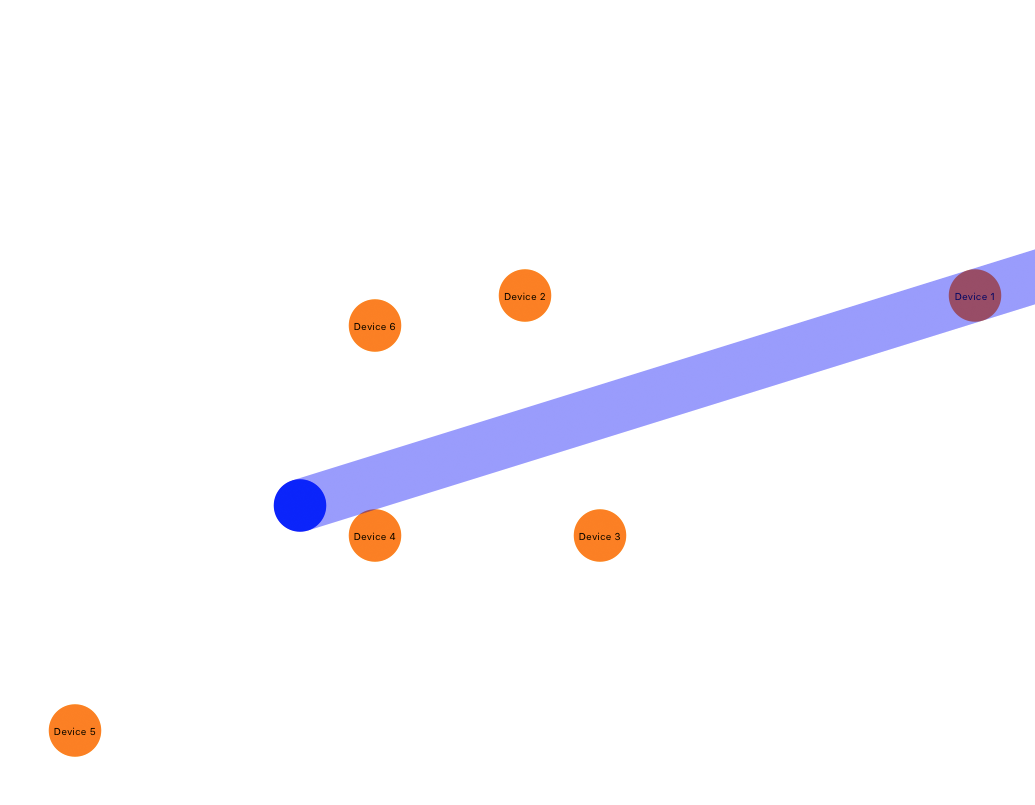
\includegraphics[width=0.3\textwidth]{images/system-correctness-initial}}
    }
    \subbottom[Accepted position of the user. Even though the user is offsetted, device 1 is still in his line of sight.]{\label{fig:evaluation:system-correctness:simulation:accepted}
        \frame{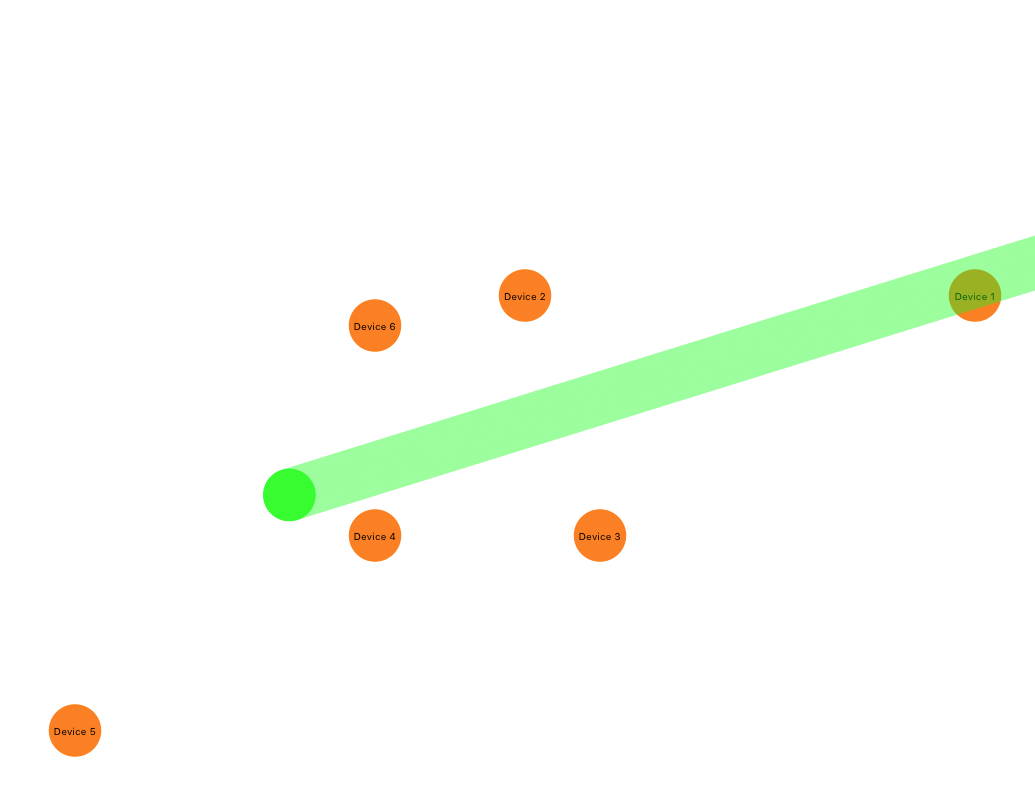
\includegraphics[width=0.3\textwidth]{images/system-correctness-accepted}}
    }
    \subbottom[Rejected position of the user. Due to the offset, device 1 is no longer in the users line of sight.]{\label{fig:evaluation:system-correctness:simulation:failure}
        \frame{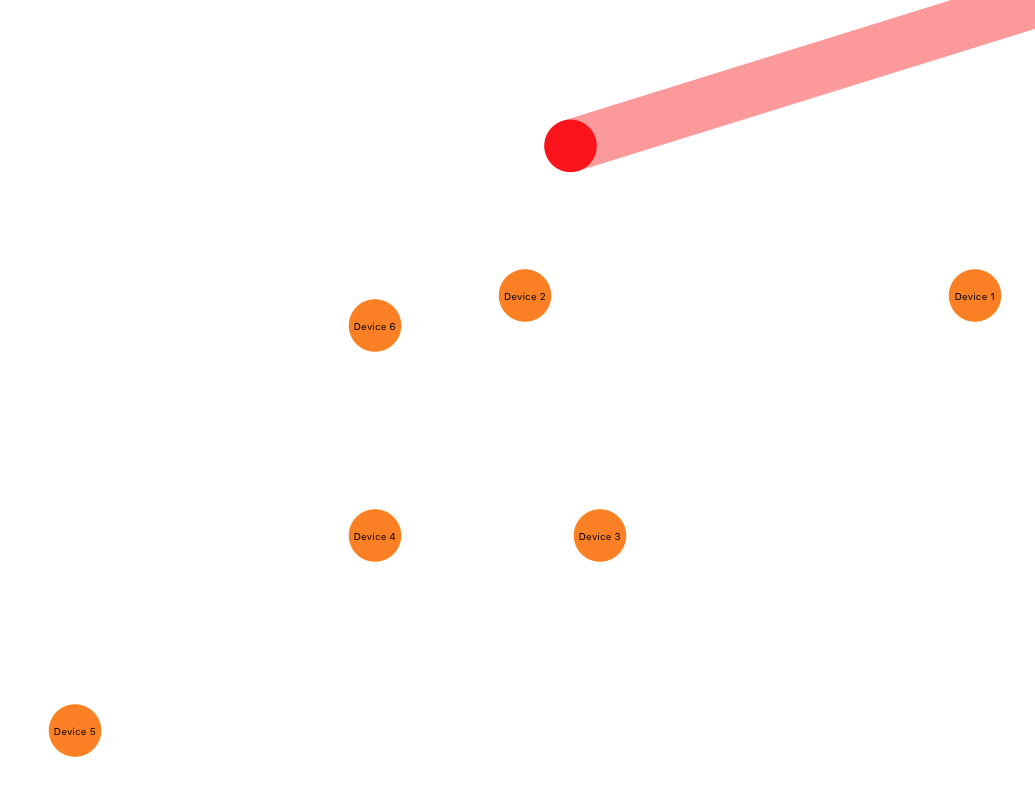
\includegraphics[width=0.3\textwidth]{images/system-correctness-failure}}
    }
    \caption{Illustrations of the simulation. Device 1 is the desired device to be focused.}
    \label{fig:evaluation:system-correctness:simulation}
\end{figure}

\subsection{Results}

Table \ref{lst:evaluation:system-correctness:results} shows the results of the simulation. We tested the system with offsets from 0 to 2.92 meters with a 0.5 meters interval. We test up to 2.92 meters as this is the average mean error we measured when testing the precision of Estimote as described in section \ref{sec:estimoteprecision}.

\begin{table}[]
\centering
\caption{Results of the seven tests performed. The ``Offset'' column shows the total offset applied to the users position and the ``Accuracy'' column shows the number of tests that resulted in the desired device being in the line of sight. The accuracy has been rounded to two decimals.}
\label{lst:evaluation:system-correctness:results}
\begin{tabular}{cc}
\textbf{Offset} & \textbf{Accuracy} \\
\hline
0 meters        & 100\%           \\
0.5 meters      & 88.93\%         \\
1 meter         & 56.67\%         \\
1.5 meters      & 23.54\%         \\
2 meters        & 12.56\%         \\
2.5 meters      & 6.89\%         \\
2.92 meters     & 4.29\%        
\end{tabular}
\end{table}

\begin{figure}[!htb]
    \centering
    \begin{tikzpicture}
  \begin{axis}[
%      ybar,
%      bar width=2pt,
      xlabel = Offset in meters,
      ylabel = Accuracy in percent,
      xtick=data,
      width=0.95\textwidth,
      height = 6cm,
      yticklabel style={align=right,inner sep=0pt,xshift=-0.3em},
      enlargelimits = false,
      ymax = 100,
      grid=major,
      try min ticks=10]]
    \addplot table[x=offset, y=accuracy] {data/system-correctness/results.csv};   
  \end{axis}
\end{tikzpicture}
    \caption{Accuracy of the system for each of the offsets in table \ref{lst:evaluation:system-correctness:results}.}
    \label{fig:evaluation:system-correctness:results}
\end{figure}

Based on the results presented in table \ref{lst:evaluation:system-correctness:results} and illustrated in figure \ref{fig:evaluation:system-correctness:results} we can conclude that the system is not sufficiently accurate. With a mean error of 2.92 meters, the system will only point at the desired device 4.29\% of the time. In order to achieve the desired accuracy described in the requirements section in section \ref{sec:requirements-specification} we must reduce the offset to 0.5 - 1 meters.

Inaccuracy in the orientation of the user, which may the result of an inaccurate magnometer, was not simulated in this test. From use through out the project we generally found the magnometer to be reliable within a few degrees. Furthermore any inaccuracy in the measurements provided by the magnometer could be compensated by a wider visibility angle.

%%% Local Variables:
%%% mode: latex
%%% TeX-master: "../../master"
%%% End:

% \section{Overall System Correctness}\label{sec:systemcorrectness}
This test is designed to test the system as a whole. 
We want to test how many times the system:
\begin{enumerate}
    \item Sends the right action to the right device
    \item Sends the wrong action to the right device
    \item Sends the right action to the wrong device
    \item Sends the wrong action to the wrong device
\end{enumerate}
Thus this test is meant to total correctness of our system. 

We have the following setup, also illustrated in \Cref{fig:totalcorrectness}:
[SETUP: Which devices, where they are, where we stand, etc.]
\begin{figure}[!htb]
    \centering
    \todo[author=Thalley]{Insert figure}
    \caption{Illustration of our setup for the total correctness test}
    \label{fig:totalcorrectness}
\end{figure}

We send a total of [NUMBER OF GESTURES]. 
\Cref{table:correctnessresults} shows the results of this test.

\begin{table}
    \centering
    \begin{tabular}{l|cc}
                     & Right action & Wrong Action \\ \hline
        Right Device &      x       &     z        \\
        Wrong Device &      y       &     w        \\
    \end{tabular} 
    
    \todo[author=Thalley]{Insert results}
    \caption{Table showing the correctness of our system}
    \label{table:correctnessresults}
\end{table}

\subsection{Overall System Correctness Conclusion}
From the results, we can conclude that... \todo[author=Thalley]{Write conclusion of precision test based on results}

\section{Conclusion}
\begin{frame}{Conclusion}{Problem Statement}
  \begin{framed}
    How can wearables be utilized for home automation in a gesture driven solution?
  \end{framed}
  
  \begin{itemize}
    \item<2-> Developed a system that can control a smart home using a wearable
    \item<2-> Utilizes BLE beacons for indoor positioning
    \item<2-> Points at the correct devices \perc{4.29} of the time
    \item<2-> However, if we exclude the numbers from Room 3, we get
    \begin{itemize}
      \item<2-> An average position accuracy of \SI{2.1}{\meter}
      \item<2-> Corresponds to \perc{\sim12.5} correctness rate
    \end{itemize}
    \item<2-> We need a position accuracy of \SI{\sim 0.6}{\meter} to meet our requirement
  \end{itemize}
\end{frame}

%Thalley: Tænker lidt at slides med de spændende future works bliver for kedelige at se på
\begin{frame}{Future Work}
  \begin{enumerate}
    \item Use a wearable
    \item Investigate Alternatives for Indoor Positioning 
    \item Include Information About the User's Context
    \item Configuration of Locations
    \item Improve Detection of Pointing
    \item Continuous Recognition of Gestures
    \item 3-Dimensional Positions
    \item Support for more than binary gestures
  \end{enumerate}
\end{frame}


\end{document}

%%% Local Variables:
%%% mode: latex
%%% TeX-master: t
%%% End:
